%chapitre1

\chapter{RIPE Atlas}

\section{Introduction}
%Le présent chapitre  introduit   le projet  RIPE Atlas. La première section est consacrée à la présentation détaillée de ce projet. La deuxième section   reprend  une liste non exhaustive de quelques outils similaires aux sondes Atlas en matière d'objectifs. La troisième section expose quelques limites du système RIPE Atlas. La dernière section reprend brièvement quelques travaux basés sur le projet RIPE Atlas.



Le présent chapitre est une présentation détaillée du projet RIPE Atlas créé par l'organisme RIPE NCC (Réseaux IP Européens - Network Coordination Centre).  RIPE Atlas  a introduit l'utilisation des dispositifs pour  effectuer des mesures des réseaux informatiques dans le monde. Ce chapitre présente dans un premier temps les caractéristiques des sondes Atlas, ensuite, il  reprend une liste non exhaustive  de quelques outils similaires aux sondes Atlas en matière d'objectifs, puis, il expose quelques limites du système RIPE Atlas. Enfin, ce chapitre  liste  brièvement quelques travaux basés sur le projet RIPE Atlas illustrant les cas d'usage de présent projet.


\section{A propos RIPE NCC}
Le RIPE NCC  est un organisme qui alloue les blocs d'adresses IP et des numéros des Systèmes Autonomes dans l'Europe et une partie de l'Asie, notamment au Moyen-Orient. 

\begin{tcolorbox}
	Un\textit{ \textbf{Système Autonome}}, appelé AS, est un ensemble de réseaux et de routeurs sous la responsabilité d'une même autorité administrative. Chaque Système Autonome est identifié par un code sur 16 bits uniques. Les protocoles qui tournent au sein d'un Système Autonome peuvent être différents.
\end{tcolorbox}

RIPE NCC assure différents services relatifs à la gestion des réseaux informatiques. Il maintient multiples projets  pour un nombre de protocoles comme DNS (Domain Name System)  (DNSMON\footnote{Source : \url{https://atlas.ripe.net/dnsmon/}, consultée le $27/12/2018$.}), BGP (Routing Information Service ou RIS\footnote{Source : \url{https://www.ripe.net/analyse/internet-measurements/routing-information-service-ris}, consultée le $27/12/2018$.}) et d'autres projets et services. En particulier, nous sommes intéressés  par le projet RIPE Atlas géré aussi par RIPE NCC. L'objectif du projet RIPE Atlas est de déployer des dispositifs dans le monde qui sont capables de collecter des données relatives aux réseaux informatiques. %Nous allons le détailler dans la section \ref{ripeatlassection}. 


\section{Présentation du projet RIPE Atlas } \label{ripeatlassection}

RIPE NCC a créé le projet RIPE Atlas en $2010$. Le nombre de sondes déployées est en augmentation constante, sachant qu'elles sont déployées par des volontaires.

\subsection{Les mesures  actives et passives de l'Internet}

Il existe plusieurs approches pour analyser l'état  d'un réseau informatique. Les deux approches les plus répandues sont~:   passive et active. L'approche passive fait référence au processus de mesure d'un réseau, sans créer ou modifier le trafic sur ce réseau.   L'approche active  repose sur l'injection des paquets  sur le réseau et surveiller le flux de ce trafic. Cette injection a pour objectif la collecte  des données relatives aux performances du réseau en question. Par exemple, la mesure du temps de réponse, le suivi du chemin des paquets, etc. 

Les données collectées permettent de surveiller les réseaux pour ensuite  proposer des améliorations de l'Internet. Le projet RIPE Atlas est un des outils s'inscrivant dans l'approche active. Ce sont  des dispositifs, appelés sondes, hébergés par des volontaires, ils sont distribués et maintenus par  RIPE NCC. Les données collectées par ces dispositifs sont disponibles au public sur le depôt de RIPE Atlas \cite{ripe-atlas-data}.

Actuellement,  plus de $10.000$ sondes Atlas sont actives, ces dernières produisent environ $450$ millions de mesures par jour, ce qui correspond à  $5,000$ résultats par seconde \cite{WinNT}.


\subsection{Généralités sur les sondes  Atlas}
\begin{itemize}
	\item[--] Les sondes Atlas  mesurent les performances de la couche IP. Une sonde  envoie des paquets réels et observe la réponse en temps réel indépendamment des applications en dessus de la couche IP.
	
	\item[--] Les sondes Atlas ne sont pas des observatrices des données comme le trafic du routage BGP, ainsi, elles n'observent pas  le trafic de leurs hébergeurs.
	
	\item[--] Les sondes  Atlas se situent dans différents emplacements dans le monde, cette répartition permet de diversifier les mesures (voir les sections des mesures  \ref{par:whatmesureripeatlas} et \ref{par:udm}). 
	
	\item[--] Les sondes Atlas sont déployées volontairement dans une maison, un bureau,  un entrepôt de données, etc.
	
	\item[--] Les mesures peuvent être lancées à tout moment et pour n'importe quelle période\footnote{Si le nombre de crédits (voir la section des crédits \ref{credits-atlas}) disponibles le permet et qu'il n'y a pas de dépassement du nombre de mesures autorisé.}.
	
	\item[--] La participation au projet RIPE Atlas est ouverte à toute personne qui s'y intéresse, cela inclut  les résultats de mesures, les outils d'analyse, l'hébergement des sondes elles-mêmes, les travaux, etc.
	
	\item[--] RIPE Atlas simule le comportement de la couche IP. Par exemple, avec RIPE Atlas, il est possible  de~:
	\begin{itemize}
		\item Suivre l'accessibilité d'une destination \footnote{Une destination représente une adresse IP.} depuis différents emplacements dans le monde et  depuis différents réseaux. Car les sondes Atlas sont réparties dans plusieurs pays et déployées dans différents réseaux.
		
		\item Étudier des problèmes du réseau remontés en effectuant des vérifications de connectivité ad-hoc via les mesures effectuées par les sondes  Atlas.
		
		\item Tester la connectivité IPv6.
		
		\item Vérifier l'infrastructure DNS.
	\end{itemize}
	
	La section  \ref{use-cases-atlas} reprend quelques cas d'utilisation  et les sujets qu'on peut étudier en se basant sur le projet  RIPE Atlas. 
\end{itemize}

\subsection{Les générations des sondes  Atlas }

Depuis leur création   en $2010$, les sondes Atlas ont connu   trois générations du matériel : \textit{v1}, \textit{v2} et \textit{v3}. Le Tableau   \ref{tab:differents-generations-probes} reprend quelques  caractérisations de ces trois générations  et  la Figure 	\ref{fig:genarations} montre le matériel utilisé  dans chaque génération.


\begin{table}[H]
	\begin{tabularx}{\textwidth}{|X|X|X|X|}
		\hline
		&\textbf{v$ 1 $}&\textbf{v$ 2 $}&\textbf{v$ 3 $} \\ \hline
		\textbf{Matériel informatique}  & Lantronix XPort Pro \cite{LantronixXPortPro} &Lantronix XPort Pro \cite{LantronixXPortPro}&tp-link tl-mr$ 3020  $  \\ \hline
		\textbf{Début d'utilisation}  &$2010$&$2011$&$2013$ \\ \hline
		\textbf{Mémoire RAM} & $8$ Mo&$16$ Mo& $32$ Mo\\ \hline
		\textbf{Mémoire Flash} & $16$ Mo&$16$ Mo&$4$ Mo \\ \hline
		\textbf{CPU} &$ 32 $-bit& $ 32 $-bit & $ 32 $-bit\\ \hline
		\textbf{Support du Wi-Fi} &Non&Non&oui \\ \hline
		\textbf{Support du NAT} &oui&oui&oui \\ \hline
		\textbf{Vitesses supportées} &$ 10 $ Mbit/s et $ 100 $ Mbit/s&$ 10 $ Mbit/s et $ 100 $ Mbit/s&$ 10 $ Mbit/s et $ 100 $ Mbit/s \\ \hline
		
	\end{tabularx}
	\caption{Les caractéristiques du matériel  des trois générations des sondes  Atlas }
	\label{tab:differents-generations-probes}
\end{table}


\begin{figure}[H]
	
	\parbox{.32\textwidth}{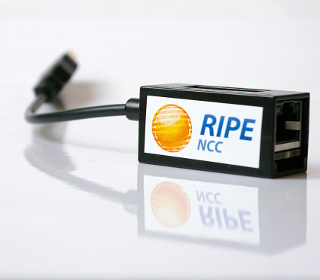
\includegraphics[width=.30\textwidth, height=.20\textwidth]{illustrations/v1} 	\captionsetup{justification=centering}\caption{Génération 1}}
	\hfill
	\parbox{.32\textwidth}{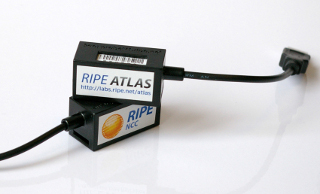
\includegraphics[width=.30\textwidth, height=.20\textwidth]{illustrations/v2}
		\captionsetup{justification=centering}
		\caption{Génération 2}}
	\hfill
	\parbox{.32\textwidth}{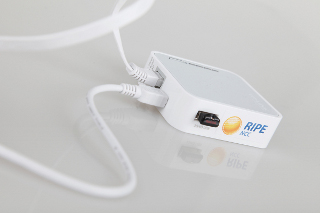
\includegraphics[width=.30\textwidth,height=.20\textwidth]{illustrations/v3} 	\captionsetup{justification=centering}\caption{Génération 3}}
	\caption{Les trois générations des sondes Atlas}
	\label{fig:genarations}
	\source{\url{https://atlas.ripe.net/docs/}, consultée le $05/08/2018$.}
\end{figure}

Pour précision, les générations $1$ et $2$ présentent une très faible consommation d'énergie, cependant, elles ont un temps de redémarrage et coûts de production élevés. 

%Pour la génération $3$, même si elle est conçue en utilisant tp-link tl-mr3020,  la sonde v3 ne sert pas comme un routeur Wi-Fi.
%, pourtant, elle a les mêmes fonctionnalités que les sondes v1 et v2.

En $2015$, plusieurs utilisateurs des sondes  Atlas ont montré un intérêt aux sondes virtuelles. Les sondes virtuelles présentent des avantages et aussi des inconvénients. Parmi les avantages, la conception des sondes virtuelles permet d'explorer des emplacements qui sont difficilement accessibles. En effet, cela permet d'étendre le réseau des sondes  Atlas. D'autre part, les sondes virtuelles peuvent être installées sans contraintes physiques ou organisationnelles. Parmi les inconvénients, une complexité sera ajoutée au système RIPE Atlas, plus de ressources seront demandées. De plus, il peut y avoir le problème de la qualité de données; le manque de données peut faire référence à une perte de paquets ou bien la machine qui héberge la sonde n'est plus disponible pour continuer les mesures. 


\subsection{Les versions du firmware des sondes Atlas} \label{subsec:firmwareversion}
En principe, toutes les sondes Atlas collectent la même information, indépendamment de leur version du firmware. On trouve les mêmes attributs\footnote{Attribut dans le sens du JSON : chaque résultat de mesure est enregistré comme étant un objet JSON.}  dans toutes les versions sauf de léger changements : ajout d'un ou de plusieurs attributs, la modification des noms des attributs, etc. Pour la simplification, nous donnons un identifiant entier pour chaque version, entre les parenthèses. Cet identifiant sera utilisé dans la suite de ce document. 

%Les résultats de mesures  sont sauvegardés dans des fichiers JSON. Chaque mesure est un tableau d'éléments. chaque élément est un tableau associative. La structure des tableau associatifs dépend de la version du firmware. \par


Il existe plusieurs versions du firmware:
\begin{itemize}
	\setlength\itemsep{0.1 cm}
	\item[--] version $1$ est identifié par  $1$ (1);
	\item[--] version $4400$  est identifiée par une valeur entre  $4400$ et $4459$ (2);
	\item[--] version $4460$ est identifiée par une valeur entre $4460$ et $4539$ (3);
	\item[--] version $4540$  est identifiée par une valeur entre  $4540$ et $4569$ (4);
	\item[--]  version $4570$  est identifiée par une valeur entre $4570$ et $4609$ (5);
	\item[--] la dernière version du firmeware \footnote{A la date de consultation $ 25/01/2018 $.} est $4610$ (6). 
\end{itemize}

\subsection{La connexion des sondes Atlas à Internet}

Les génération $1$ et $2$ des sondes  Atlas ont une interface Ethernet (RJ-45). La génération $3$ dispose techniquement des capacités Wi-Fi. Cependant, ces sondes ne sont pas suffisamment prêtes au niveau logiciel pour supporter le Wi-Fi.
% L'objectif était de garder l'indépendance des sondes Atlas du trafic de celui qui les héberge.

Une fois la sonde se connecte au port d'Ethernet, elle acquiert  une adresse IPv4, un résolveur DNS  en utilisant DHCP et la configuration IPv6 via \textit{Router Advertisement}. Ensuite, elle essaie de rejoindre l'infrastructure du RIPE Atlas. Pour ce faire, elle utilise le résolveur DNS et se connecte à l'infrastructure à travers SSH sur le port TCP de sortie $443$ comme il est illustré dans la Figure \ref{fig:ssh-atlas-probe}. L'architecture du système RIPE Atlas est détaillée dans la section \ref{subsec:archi-probes}.

\begin{figure}[H]
	\centering
	\captionsetup{justification=centering}
	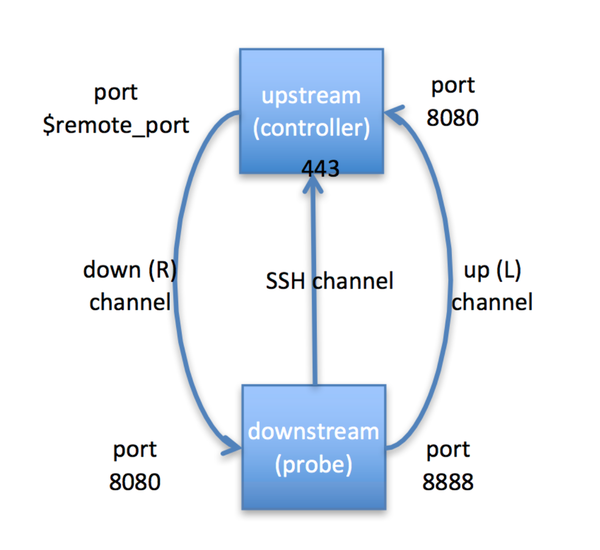
\includegraphics[width=0.5\linewidth]{illustrations/ssh-atlas-probe}
	\caption{La connexion des sondes Atlas à l'infrastructure RIPE Atlas \cite{how-we-manage-our-probe}}
	\label{fig:ssh-atlas-probe}
\end{figure}

\subsection{Architecture du système RIPE Atlas} \label{subsec:archi-probes}

Il existe deux catégories d'outils de surveillance du réseau: des outils matériels et d'autres logiciels. Les sondes  Atlas sont parmi les outils matériels. Le choix d'utilisation d'un outil matériel au lieu d'un outil logiciel dépend de plusieurs facteurs, par exemple l'indépendance du système d'exploitation, la facilité de déploiement, la disponibilité des sondes tout le temps (au lieu d'être dépendante de la machine qui l'héberge) et d'autres facteurs liés à la sécurité.

Le système RIPE Atlas est conçu pour qu'il soit opérationnel de façon distribuée. La plupart des composantes ont assez de connaissances pour remplir leurs rôles, sans nécessairement avoir besoin de connaître les états des autres composantes du système. Cela assure que le système soit capable d'assurer la plupart des fonctionnalités en cas  d'un problème temporaire. Par exemple, si une sonde est déconnectée de l'infrastructure, elle continue les mesures planifiées et les données sont renvoyées dès sa reconnexion au système.


La Figure  \ref{fig:archi-ripe-atlas} montre une vue d'ensemble de l'architecture du RIPE Atlas.

\begin{figure}[H]
	\centering
	\resizebox{\textwidth}{!}{
		% Graphic for TeX using PGF
% Title: /home/bellafkih/Documents/2017-2018/Mémoire/report_memoire/illustrations/Diagramme1.dia
% Creator: Dia v0.97.3
% CreationDate: Thu Mar  1 16:26:10 2018
% For: bellafkih
% \usepackage{tikz}
% The following commands are not supported in PSTricks at present
% We define them conditionally, so when they are implemented,
% this pgf file will use them.
\ifx\du\undefined
  \newlength{\du}
\fi
\setlength{\du}{15\unitlength}
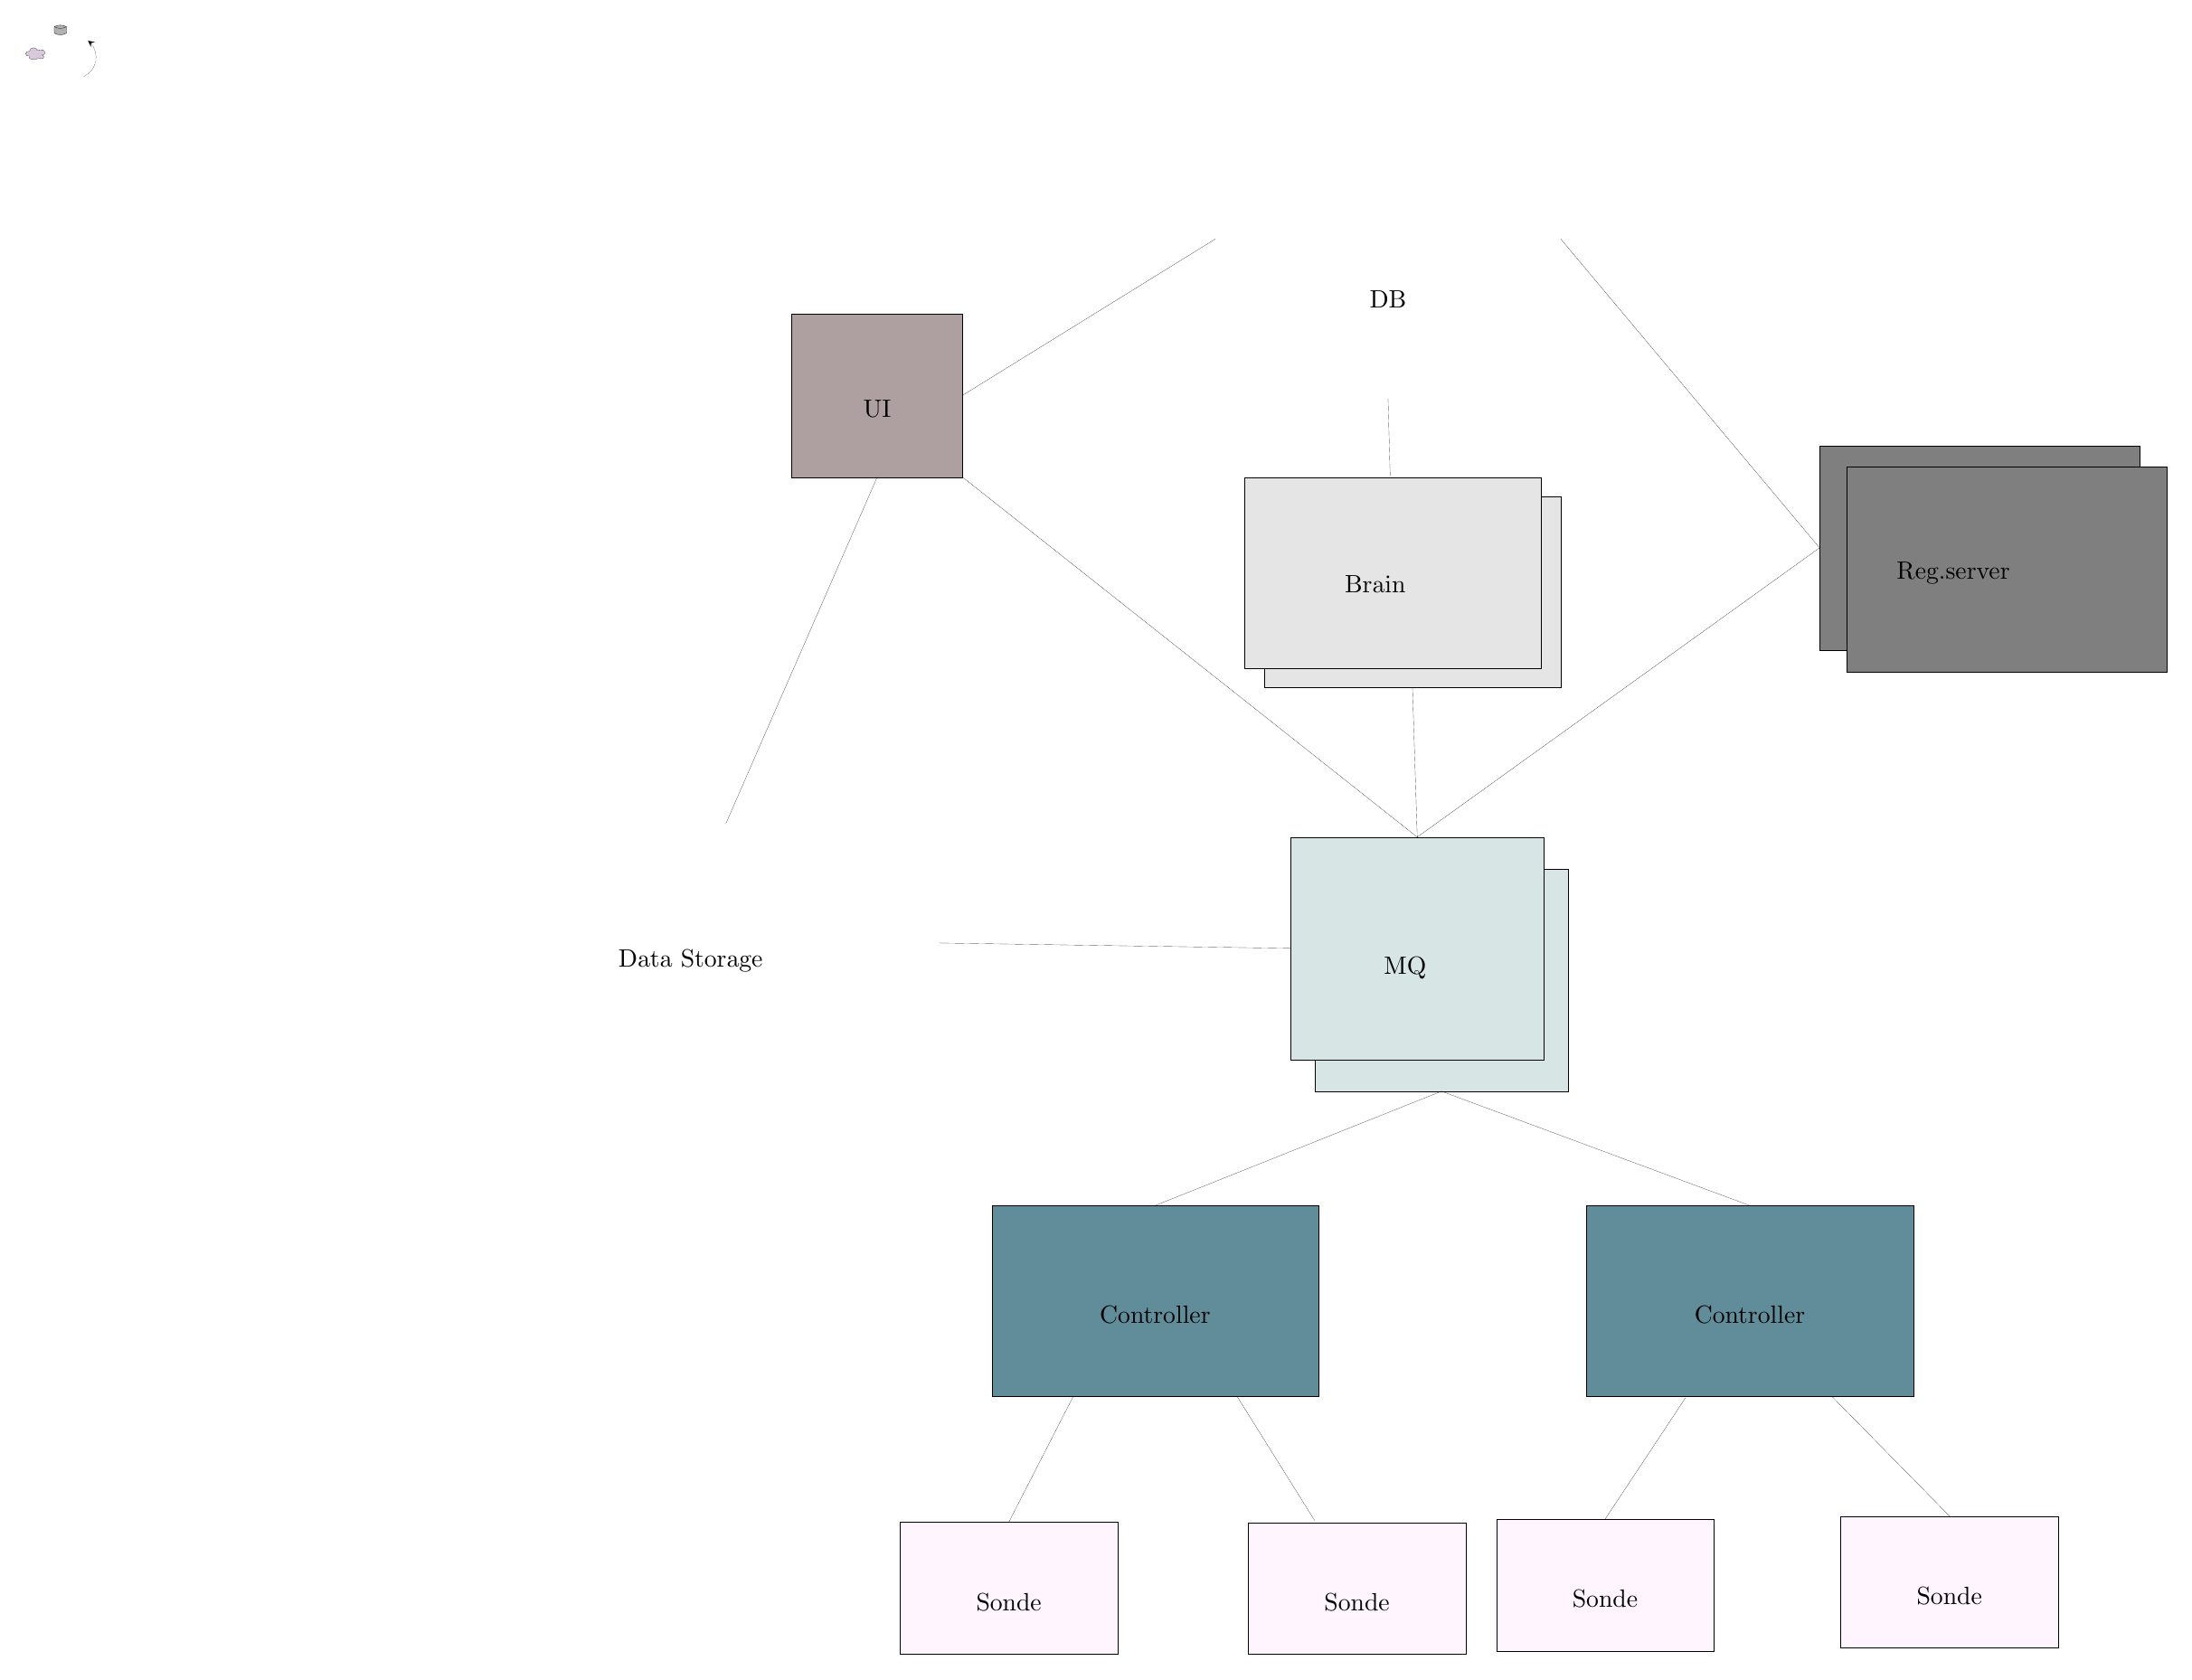
\begin{tikzpicture}
\pgftransformxscale{1.000000}
\pgftransformyscale{-1.000000}
\definecolor{dialinecolor}{rgb}{0.000000, 0.000000, 0.000000}
\pgfsetstrokecolor{dialinecolor}
\definecolor{dialinecolor}{rgb}{1.000000, 1.000000, 1.000000}
\pgfsetfillcolor{dialinecolor}
\pgfsetlinewidth{0.100000\du}
\pgfsetdash{}{0pt}
\pgfsetdash{}{0pt}
\pgfsetbuttcap
\pgfsetmiterjoin
\pgfsetlinewidth{0.100000\du}
\pgfsetbuttcap
\pgfsetmiterjoin
\pgfsetdash{}{0pt}
\definecolor{dialinecolor}{rgb}{0.698039, 0.690196, 0.690196}
\pgfsetfillcolor{dialinecolor}
\pgfpathmoveto{\pgfpoint{16.900000\du}{2.091667\du}}
\pgfpathcurveto{\pgfpoint{17.870000\du}{1.610417\du}}{\pgfpoint{18.355000\du}{1.450000\du}}{\pgfpoint{19.325000\du}{1.450000\du}}
\pgfpathcurveto{\pgfpoint{20.295000\du}{1.450000\du}}{\pgfpoint{20.780000\du}{1.610417\du}}{\pgfpoint{21.750000\du}{2.091667\du}}
\pgfpathlineto{\pgfpoint{21.750000\du}{4.658333\du}}
\pgfpathcurveto{\pgfpoint{20.780000\du}{5.139583\du}}{\pgfpoint{20.295000\du}{5.300000\du}}{\pgfpoint{19.325000\du}{5.300000\du}}
\pgfpathcurveto{\pgfpoint{18.355000\du}{5.300000\du}}{\pgfpoint{17.870000\du}{5.139583\du}}{\pgfpoint{16.900000\du}{4.658333\du}}
\pgfpathlineto{\pgfpoint{16.900000\du}{2.091667\du}}
\pgfusepath{fill}
\definecolor{dialinecolor}{rgb}{0.000000, 0.000000, 0.000000}
\pgfsetstrokecolor{dialinecolor}
\pgfpathmoveto{\pgfpoint{16.900000\du}{2.091667\du}}
\pgfpathcurveto{\pgfpoint{17.870000\du}{1.610417\du}}{\pgfpoint{18.355000\du}{1.450000\du}}{\pgfpoint{19.325000\du}{1.450000\du}}
\pgfpathcurveto{\pgfpoint{20.295000\du}{1.450000\du}}{\pgfpoint{20.780000\du}{1.610417\du}}{\pgfpoint{21.750000\du}{2.091667\du}}
\pgfpathlineto{\pgfpoint{21.750000\du}{4.658333\du}}
\pgfpathcurveto{\pgfpoint{20.780000\du}{5.139583\du}}{\pgfpoint{20.295000\du}{5.300000\du}}{\pgfpoint{19.325000\du}{5.300000\du}}
\pgfpathcurveto{\pgfpoint{18.355000\du}{5.300000\du}}{\pgfpoint{17.870000\du}{5.139583\du}}{\pgfpoint{16.900000\du}{4.658333\du}}
\pgfpathlineto{\pgfpoint{16.900000\du}{2.091667\du}}
\pgfusepath{stroke}
\pgfsetbuttcap
\pgfsetmiterjoin
\pgfsetdash{}{0pt}
\definecolor{dialinecolor}{rgb}{0.000000, 0.000000, 0.000000}
\pgfsetstrokecolor{dialinecolor}
\pgfpathmoveto{\pgfpoint{16.900000\du}{2.091667\du}}
\pgfpathcurveto{\pgfpoint{17.870000\du}{2.572917\du}}{\pgfpoint{18.355000\du}{2.733333\du}}{\pgfpoint{19.325000\du}{2.733333\du}}
\pgfpathcurveto{\pgfpoint{20.295000\du}{2.733333\du}}{\pgfpoint{20.780000\du}{2.572917\du}}{\pgfpoint{21.750000\du}{2.091667\du}}
\pgfusepath{stroke}
% setfont left to latex
\definecolor{dialinecolor}{rgb}{0.000000, 0.000000, 0.000000}
\pgfsetstrokecolor{dialinecolor}
\node at (19.325000\du,3.895833\du){DB};
\definecolor{dialinecolor}{rgb}{0.682353, 0.627451, 0.627451}
\pgfsetfillcolor{dialinecolor}
\fill (10.950000\du,4.100000\du)--(10.950000\du,6.400000\du)--(13.350000\du,6.400000\du)--(13.350000\du,4.100000\du)--cycle;
\pgfsetlinewidth{0.100000\du}
\pgfsetdash{}{0pt}
\pgfsetdash{}{0pt}
\pgfsetmiterjoin
\definecolor{dialinecolor}{rgb}{0.000000, 0.000000, 0.000000}
\pgfsetstrokecolor{dialinecolor}
\draw (10.950000\du,4.100000\du)--(10.950000\du,6.400000\du)--(13.350000\du,6.400000\du)--(13.350000\du,4.100000\du)--cycle;
% setfont left to latex
\definecolor{dialinecolor}{rgb}{0.000000, 0.000000, 0.000000}
\pgfsetstrokecolor{dialinecolor}
\node at (12.150000\du,5.445000\du){UI};
\definecolor{dialinecolor}{rgb}{0.898039, 0.898039, 0.898039}
\pgfsetfillcolor{dialinecolor}
\fill (17.586250\du,6.675000\du)--(17.586250\du,9.350000\du)--(21.750000\du,9.350000\du)--(21.750000\du,6.675000\du)--cycle;
\pgfsetlinewidth{0.050000\du}
\pgfsetdash{}{0pt}
\pgfsetdash{}{0pt}
\pgfsetmiterjoin
\definecolor{dialinecolor}{rgb}{0.000000, 0.000000, 0.000000}
\pgfsetstrokecolor{dialinecolor}
\draw (17.586250\du,6.675000\du)--(17.586250\du,9.350000\du)--(21.750000\du,9.350000\du)--(21.750000\du,6.675000\du)--cycle;
% setfont left to latex
\definecolor{dialinecolor}{rgb}{0.000000, 0.000000, 0.000000}
\pgfsetstrokecolor{dialinecolor}
\node at (19.668125\du,8.207500\du){};
\definecolor{dialinecolor}{rgb}{0.898039, 0.898039, 0.898039}
\pgfsetfillcolor{dialinecolor}
\fill (17.310000\du,6.405000\du)--(17.310000\du,9.080000\du)--(21.473750\du,9.080000\du)--(21.473750\du,6.405000\du)--cycle;
\pgfsetlinewidth{0.050000\du}
\pgfsetdash{}{0pt}
\pgfsetdash{}{0pt}
\pgfsetmiterjoin
\definecolor{dialinecolor}{rgb}{0.000000, 0.000000, 0.000000}
\pgfsetstrokecolor{dialinecolor}
\draw (17.310000\du,6.405000\du)--(17.310000\du,9.080000\du)--(21.473750\du,9.080000\du)--(21.473750\du,6.405000\du)--cycle;
% setfont left to latex
\definecolor{dialinecolor}{rgb}{0.000000, 0.000000, 0.000000}
\pgfsetstrokecolor{dialinecolor}
\node at (19.391875\du,7.937500\du){};
\definecolor{dialinecolor}{rgb}{0.498039, 0.498039, 0.498039}
\pgfsetfillcolor{dialinecolor}
\fill (25.385000\du,5.955000\du)--(25.385000\du,8.830000\du)--(29.885000\du,8.830000\du)--(29.885000\du,5.955000\du)--cycle;
\pgfsetlinewidth{0.050000\du}
\pgfsetdash{}{0pt}
\pgfsetdash{}{0pt}
\pgfsetmiterjoin
\definecolor{dialinecolor}{rgb}{0.000000, 0.000000, 0.000000}
\pgfsetstrokecolor{dialinecolor}
\draw (25.385000\du,5.955000\du)--(25.385000\du,8.830000\du)--(29.885000\du,8.830000\du)--(29.885000\du,5.955000\du)--cycle;
% setfont left to latex
\definecolor{dialinecolor}{rgb}{0.000000, 0.000000, 0.000000}
\pgfsetstrokecolor{dialinecolor}
\node at (27.635000\du,7.587500\du){};
\definecolor{dialinecolor}{rgb}{0.498039, 0.498039, 0.498039}
\pgfsetfillcolor{dialinecolor}
\fill (25.760000\du,6.255000\du)--(25.760000\du,9.130000\du)--(30.260000\du,9.130000\du)--(30.260000\du,6.255000\du)--cycle;
\pgfsetlinewidth{0.050000\du}
\pgfsetdash{}{0pt}
\pgfsetdash{}{0pt}
\pgfsetmiterjoin
\definecolor{dialinecolor}{rgb}{0.000000, 0.000000, 0.000000}
\pgfsetstrokecolor{dialinecolor}
\draw (25.760000\du,6.255000\du)--(25.760000\du,9.130000\du)--(30.260000\du,9.130000\du)--(30.260000\du,6.255000\du)--cycle;
% setfont left to latex
\definecolor{dialinecolor}{rgb}{0.000000, 0.000000, 0.000000}
\pgfsetstrokecolor{dialinecolor}
\node at (28.010000\du,7.887500\du){};
\definecolor{dialinecolor}{rgb}{0.847059, 0.898039, 0.898039}
\pgfsetfillcolor{dialinecolor}
\fill (18.300000\du,11.900000\du)--(18.300000\du,15.025000\du)--(21.850000\du,15.025000\du)--(21.850000\du,11.900000\du)--cycle;
\pgfsetlinewidth{0.050000\du}
\pgfsetdash{}{0pt}
\pgfsetdash{}{0pt}
\pgfsetmiterjoin
\definecolor{dialinecolor}{rgb}{0.000000, 0.000000, 0.000000}
\pgfsetstrokecolor{dialinecolor}
\draw (18.300000\du,11.900000\du)--(18.300000\du,15.025000\du)--(21.850000\du,15.025000\du)--(21.850000\du,11.900000\du)--cycle;
% setfont left to latex
\definecolor{dialinecolor}{rgb}{0.000000, 0.000000, 0.000000}
\pgfsetstrokecolor{dialinecolor}
\node at (20.075000\du,13.657500\du){};
\definecolor{dialinecolor}{rgb}{0.847059, 0.898039, 0.898039}
\pgfsetfillcolor{dialinecolor}
\fill (17.960000\du,11.455000\du)--(17.960000\du,14.580000\du)--(21.510000\du,14.580000\du)--(21.510000\du,11.455000\du)--cycle;
\pgfsetlinewidth{0.050000\du}
\pgfsetdash{}{0pt}
\pgfsetdash{}{0pt}
\pgfsetmiterjoin
\definecolor{dialinecolor}{rgb}{0.000000, 0.000000, 0.000000}
\pgfsetstrokecolor{dialinecolor}
\draw (17.960000\du,11.455000\du)--(17.960000\du,14.580000\du)--(21.510000\du,14.580000\du)--(21.510000\du,11.455000\du)--cycle;
% setfont left to latex
\definecolor{dialinecolor}{rgb}{0.000000, 0.000000, 0.000000}
\pgfsetstrokecolor{dialinecolor}
\node at (19.735000\du,13.212500\du){};
\pgfsetlinewidth{0.050000\du}
\pgfsetdash{}{0pt}
\pgfsetdash{}{0pt}
\pgfsetbuttcap
\pgfsetmiterjoin
\pgfsetlinewidth{0.050000\du}
\pgfsetbuttcap
\pgfsetmiterjoin
\pgfsetdash{}{0pt}
\definecolor{dialinecolor}{rgb}{0.854902, 0.788235, 0.854902}
\pgfsetfillcolor{dialinecolor}
\pgfpathmoveto{\pgfpoint{7.085270\du}{11.834673\du}}
\pgfpathcurveto{\pgfpoint{6.451876\du}{11.817409\du}}{\pgfpoint{5.223477\du}{12.179945\du}}{\pgfpoint{5.396221\du}{12.956808\du}}
\pgfpathcurveto{\pgfpoint{5.568963\du}{13.733671\du}}{\pgfpoint{6.394295\du}{13.906300\du}}{\pgfpoint{6.739782\du}{13.681880\du}}
\pgfpathcurveto{\pgfpoint{7.085270\du}{13.457453\du}}{\pgfpoint{6.202357\du}{14.769481\du}}{\pgfpoint{7.891408\du}{15.114754\du}}
\pgfpathcurveto{\pgfpoint{9.580443\du}{15.460026\du}}{\pgfpoint{10.444162\du}{14.907590\du}}{\pgfpoint{10.194643\du}{14.510527\du}}
\pgfpathcurveto{\pgfpoint{9.945124\du}{14.113464\du}}{\pgfpoint{11.672562\du}{15.442763\du}}{\pgfpoint{12.478700\du}{14.683163\du}}
\pgfpathcurveto{\pgfpoint{13.284837\du}{13.923564\du}}{\pgfpoint{11.653368\du}{13.198499\du}}{\pgfpoint{11.998856\du}{13.302081\du}}
\pgfpathcurveto{\pgfpoint{12.344343\du}{13.405662\du}}{\pgfpoint{13.400000\du}{13.267553\du}}{\pgfpoint{13.054512\du}{11.972782\du}}
\pgfpathcurveto{\pgfpoint{12.709025\du}{10.678010\du}}{\pgfpoint{9.599636\du}{11.679300\du}}{\pgfpoint{9.945124\du}{11.489401\du}}
\pgfpathcurveto{\pgfpoint{10.290612\du}{11.299501\du}}{\pgfpoint{9.426893\du}{10.350000\du}}{\pgfpoint{8.352058\du}{10.539900\du}}
\pgfpathcurveto{\pgfpoint{7.277207\du}{10.729801\du}}{\pgfpoint{7.200970\du}{11.074400\du}}{\pgfpoint{7.085807\du}{11.834000\du}}
\pgfpathlineto{\pgfpoint{7.085270\du}{11.834673\du}}
\pgfusepath{fill}
\definecolor{dialinecolor}{rgb}{0.000000, 0.000000, 0.000000}
\pgfsetstrokecolor{dialinecolor}
\pgfpathmoveto{\pgfpoint{7.085270\du}{11.834673\du}}
\pgfpathcurveto{\pgfpoint{6.451876\du}{11.817409\du}}{\pgfpoint{5.223477\du}{12.179945\du}}{\pgfpoint{5.396221\du}{12.956808\du}}
\pgfpathcurveto{\pgfpoint{5.568963\du}{13.733671\du}}{\pgfpoint{6.394295\du}{13.906300\du}}{\pgfpoint{6.739782\du}{13.681880\du}}
\pgfpathcurveto{\pgfpoint{7.085270\du}{13.457453\du}}{\pgfpoint{6.202357\du}{14.769481\du}}{\pgfpoint{7.891408\du}{15.114754\du}}
\pgfpathcurveto{\pgfpoint{9.580443\du}{15.460026\du}}{\pgfpoint{10.444162\du}{14.907590\du}}{\pgfpoint{10.194643\du}{14.510527\du}}
\pgfpathcurveto{\pgfpoint{9.945124\du}{14.113464\du}}{\pgfpoint{11.672562\du}{15.442763\du}}{\pgfpoint{12.478700\du}{14.683163\du}}
\pgfpathcurveto{\pgfpoint{13.284837\du}{13.923564\du}}{\pgfpoint{11.653368\du}{13.198499\du}}{\pgfpoint{11.998856\du}{13.302081\du}}
\pgfpathcurveto{\pgfpoint{12.344343\du}{13.405662\du}}{\pgfpoint{13.400000\du}{13.267553\du}}{\pgfpoint{13.054512\du}{11.972782\du}}
\pgfpathcurveto{\pgfpoint{12.709025\du}{10.678010\du}}{\pgfpoint{9.599636\du}{11.679300\du}}{\pgfpoint{9.945124\du}{11.489401\du}}
\pgfpathcurveto{\pgfpoint{10.290612\du}{11.299501\du}}{\pgfpoint{9.426893\du}{10.350000\du}}{\pgfpoint{8.352058\du}{10.539900\du}}
\pgfpathcurveto{\pgfpoint{7.277207\du}{10.729801\du}}{\pgfpoint{7.200970\du}{11.074400\du}}{\pgfpoint{7.085807\du}{11.834000\du}}
\pgfpathlineto{\pgfpoint{7.085270\du}{11.834673\du}}
\pgfusepath{stroke}
% setfont left to latex
\definecolor{dialinecolor}{rgb}{0.000000, 0.000000, 0.000000}
\pgfsetstrokecolor{dialinecolor}
\node at (9.530923\du,13.195092\du){Data Storage};
\definecolor{dialinecolor}{rgb}{0.380392, 0.549020, 0.603922}
\pgfsetfillcolor{dialinecolor}
\fill (22.111250\du,16.630000\du)--(22.111250\du,19.305000\du)--(26.700000\du,19.305000\du)--(26.700000\du,16.630000\du)--cycle;
\pgfsetlinewidth{0.050000\du}
\pgfsetdash{}{0pt}
\pgfsetdash{}{0pt}
\pgfsetmiterjoin
\definecolor{dialinecolor}{rgb}{0.000000, 0.000000, 0.000000}
\pgfsetstrokecolor{dialinecolor}
\draw (22.111250\du,16.630000\du)--(22.111250\du,19.305000\du)--(26.700000\du,19.305000\du)--(26.700000\du,16.630000\du)--cycle;
% setfont left to latex
\definecolor{dialinecolor}{rgb}{0.000000, 0.000000, 0.000000}
\pgfsetstrokecolor{dialinecolor}
\node at (24.405625\du,18.162500\du){Controller};
\definecolor{dialinecolor}{rgb}{0.380392, 0.549020, 0.603922}
\pgfsetfillcolor{dialinecolor}
\fill (13.760000\du,16.630000\du)--(13.760000\du,19.305000\du)--(18.348750\du,19.305000\du)--(18.348750\du,16.630000\du)--cycle;
\pgfsetlinewidth{0.050000\du}
\pgfsetdash{}{0pt}
\pgfsetdash{}{0pt}
\pgfsetmiterjoin
\definecolor{dialinecolor}{rgb}{0.000000, 0.000000, 0.000000}
\pgfsetstrokecolor{dialinecolor}
\draw (13.760000\du,16.630000\du)--(13.760000\du,19.305000\du)--(18.348750\du,19.305000\du)--(18.348750\du,16.630000\du)--cycle;
% setfont left to latex
\definecolor{dialinecolor}{rgb}{0.000000, 0.000000, 0.000000}
\pgfsetstrokecolor{dialinecolor}
\node at (16.054375\du,18.162500\du){Controller};
\definecolor{dialinecolor}{rgb}{0.996078, 0.960784, 1.000000}
\pgfsetfillcolor{dialinecolor}
\fill (12.471250\du,21.075000\du)--(12.471250\du,22.925000\du)--(15.528750\du,22.925000\du)--(15.528750\du,21.075000\du)--cycle;
\pgfsetlinewidth{0.050000\du}
\pgfsetdash{}{0pt}
\pgfsetdash{}{0pt}
\pgfsetmiterjoin
\definecolor{dialinecolor}{rgb}{0.000000, 0.000000, 0.000000}
\pgfsetstrokecolor{dialinecolor}
\draw (12.471250\du,21.075000\du)--(12.471250\du,22.925000\du)--(15.528750\du,22.925000\du)--(15.528750\du,21.075000\du)--cycle;
% setfont left to latex
\definecolor{dialinecolor}{rgb}{0.000000, 0.000000, 0.000000}
\pgfsetstrokecolor{dialinecolor}
\node at (14.000000\du,22.195000\du){Sonde};
\definecolor{dialinecolor}{rgb}{0.996078, 0.960784, 1.000000}
\pgfsetfillcolor{dialinecolor}
\fill (17.360000\du,21.080000\du)--(17.360000\du,22.930000\du)--(20.417500\du,22.930000\du)--(20.417500\du,21.080000\du)--cycle;
\pgfsetlinewidth{0.050000\du}
\pgfsetdash{}{0pt}
\pgfsetdash{}{0pt}
\pgfsetmiterjoin
\definecolor{dialinecolor}{rgb}{0.000000, 0.000000, 0.000000}
\pgfsetstrokecolor{dialinecolor}
\draw (17.360000\du,21.080000\du)--(17.360000\du,22.930000\du)--(20.417500\du,22.930000\du)--(20.417500\du,21.080000\du)--cycle;
% setfont left to latex
\definecolor{dialinecolor}{rgb}{0.000000, 0.000000, 0.000000}
\pgfsetstrokecolor{dialinecolor}
\node at (18.888750\du,22.200000\du){Sonde};
\definecolor{dialinecolor}{rgb}{0.996078, 0.960784, 1.000000}
\pgfsetfillcolor{dialinecolor}
\fill (20.845000\du,21.035000\du)--(20.845000\du,22.885000\du)--(23.902500\du,22.885000\du)--(23.902500\du,21.035000\du)--cycle;
\pgfsetlinewidth{0.050000\du}
\pgfsetdash{}{0pt}
\pgfsetdash{}{0pt}
\pgfsetmiterjoin
\definecolor{dialinecolor}{rgb}{0.000000, 0.000000, 0.000000}
\pgfsetstrokecolor{dialinecolor}
\draw (20.845000\du,21.035000\du)--(20.845000\du,22.885000\du)--(23.902500\du,22.885000\du)--(23.902500\du,21.035000\du)--cycle;
% setfont left to latex
\definecolor{dialinecolor}{rgb}{0.000000, 0.000000, 0.000000}
\pgfsetstrokecolor{dialinecolor}
\node at (22.373750\du,22.155000\du){Sonde};
\definecolor{dialinecolor}{rgb}{0.996078, 0.960784, 1.000000}
\pgfsetfillcolor{dialinecolor}
\fill (25.680000\du,20.990000\du)--(25.680000\du,22.840000\du)--(28.737500\du,22.840000\du)--(28.737500\du,20.990000\du)--cycle;
\pgfsetlinewidth{0.050000\du}
\pgfsetdash{}{0pt}
\pgfsetdash{}{0pt}
\pgfsetmiterjoin
\definecolor{dialinecolor}{rgb}{0.000000, 0.000000, 0.000000}
\pgfsetstrokecolor{dialinecolor}
\draw (25.680000\du,20.990000\du)--(25.680000\du,22.840000\du)--(28.737500\du,22.840000\du)--(28.737500\du,20.990000\du)--cycle;
% setfont left to latex
\definecolor{dialinecolor}{rgb}{0.000000, 0.000000, 0.000000}
\pgfsetstrokecolor{dialinecolor}
\node at (27.208750\du,22.110000\du){Sonde};
% setfont left to latex
\definecolor{dialinecolor}{rgb}{0.000000, 0.000000, 0.000000}
\pgfsetstrokecolor{dialinecolor}
\node[anchor=west] at (26.350000\du,7.750000\du){Reg.server};
\pgfsetlinewidth{0.050000\du}
\pgfsetdash{}{0pt}
\pgfsetdash{}{0pt}
\pgfsetbuttcap
{
\definecolor{dialinecolor}{rgb}{0.000000, 0.000000, 0.000000}
\pgfsetfillcolor{dialinecolor}
% was here!!!
\definecolor{dialinecolor}{rgb}{0.000000, 0.000000, 0.000000}
\pgfsetstrokecolor{dialinecolor}
\draw (21.750000\du,3.054167\du)--(25.385000\du,7.392500\du);
}
\pgfsetlinewidth{0.050000\du}
\pgfsetdash{}{0pt}
\pgfsetdash{}{0pt}
\pgfsetbuttcap
{
\definecolor{dialinecolor}{rgb}{0.000000, 0.000000, 0.000000}
\pgfsetfillcolor{dialinecolor}
% was here!!!
\definecolor{dialinecolor}{rgb}{0.000000, 0.000000, 0.000000}
\pgfsetstrokecolor{dialinecolor}
\draw (13.350000\du,5.250000\du)--(16.900000\du,3.054167\du);
}
% setfont left to latex
\definecolor{dialinecolor}{rgb}{0.000000, 0.000000, 0.000000}
\pgfsetstrokecolor{dialinecolor}
\node[anchor=west] at (18.600000\du,7.900000\du){Brain};
\pgfsetlinewidth{0.050000\du}
\pgfsetdash{}{0pt}
\pgfsetdash{}{0pt}
\pgfsetbuttcap
{
\definecolor{dialinecolor}{rgb}{0.000000, 0.000000, 0.000000}
\pgfsetfillcolor{dialinecolor}
% was here!!!
\definecolor{dialinecolor}{rgb}{0.000000, 0.000000, 0.000000}
\pgfsetstrokecolor{dialinecolor}
\draw (19.325000\du,5.300000\du)--(19.354568\du,6.379924\du);
}
% setfont left to latex
\definecolor{dialinecolor}{rgb}{0.000000, 0.000000, 0.000000}
\pgfsetstrokecolor{dialinecolor}
\node[anchor=west] at (19.150000\du,13.300000\du){MQ};
\pgfsetlinewidth{0.050000\du}
\pgfsetdash{}{0pt}
\pgfsetdash{}{0pt}
\pgfsetbuttcap
{
\definecolor{dialinecolor}{rgb}{0.000000, 0.000000, 0.000000}
\pgfsetfillcolor{dialinecolor}
% was here!!!
\definecolor{dialinecolor}{rgb}{0.000000, 0.000000, 0.000000}
\pgfsetstrokecolor{dialinecolor}
\draw (19.668125\du,9.350000\du)--(19.735000\du,11.455000\du);
}
\pgfsetlinewidth{0.050000\du}
\pgfsetdash{}{0pt}
\pgfsetdash{}{0pt}
\pgfsetbuttcap
{
\definecolor{dialinecolor}{rgb}{0.000000, 0.000000, 0.000000}
\pgfsetfillcolor{dialinecolor}
% was here!!!
\definecolor{dialinecolor}{rgb}{0.000000, 0.000000, 0.000000}
\pgfsetstrokecolor{dialinecolor}
\draw (10.026768\du,11.262769\du)--(12.150000\du,6.400000\du);
}
\pgfsetlinewidth{0.050000\du}
\pgfsetdash{}{0pt}
\pgfsetdash{}{0pt}
\pgfsetbuttcap
{
\definecolor{dialinecolor}{rgb}{0.000000, 0.000000, 0.000000}
\pgfsetfillcolor{dialinecolor}
% was here!!!
\definecolor{dialinecolor}{rgb}{0.000000, 0.000000, 0.000000}
\pgfsetstrokecolor{dialinecolor}
\draw (13.015462\du,12.942453\du)--(17.960000\du,13.017500\du);
}
\pgfsetlinewidth{0.050000\du}
\pgfsetdash{}{0pt}
\pgfsetdash{}{0pt}
\pgfsetbuttcap
{
\definecolor{dialinecolor}{rgb}{0.000000, 0.000000, 0.000000}
\pgfsetfillcolor{dialinecolor}
% was here!!!
\definecolor{dialinecolor}{rgb}{0.000000, 0.000000, 0.000000}
\pgfsetstrokecolor{dialinecolor}
\draw (20.075000\du,15.025000\du)--(24.405625\du,16.630000\du);
}
\pgfsetlinewidth{0.050000\du}
\pgfsetdash{}{0pt}
\pgfsetdash{}{0pt}
\pgfsetbuttcap
{
\definecolor{dialinecolor}{rgb}{0.000000, 0.000000, 0.000000}
\pgfsetfillcolor{dialinecolor}
% was here!!!
\definecolor{dialinecolor}{rgb}{0.000000, 0.000000, 0.000000}
\pgfsetstrokecolor{dialinecolor}
\draw (20.075000\du,15.025000\du)--(16.054375\du,16.630000\du);
}
\pgfsetlinewidth{0.050000\du}
\pgfsetdash{}{0pt}
\pgfsetdash{}{0pt}
\pgfsetbuttcap
{
\definecolor{dialinecolor}{rgb}{0.000000, 0.000000, 0.000000}
\pgfsetfillcolor{dialinecolor}
% was here!!!
\definecolor{dialinecolor}{rgb}{0.000000, 0.000000, 0.000000}
\pgfsetstrokecolor{dialinecolor}
\draw (14.907187\du,19.305000\du)--(14.000000\du,21.075000\du);
}
\pgfsetlinewidth{0.050000\du}
\pgfsetdash{}{0pt}
\pgfsetdash{}{0pt}
\pgfsetbuttcap
{
\definecolor{dialinecolor}{rgb}{0.000000, 0.000000, 0.000000}
\pgfsetfillcolor{dialinecolor}
% was here!!!
\definecolor{dialinecolor}{rgb}{0.000000, 0.000000, 0.000000}
\pgfsetstrokecolor{dialinecolor}
\draw (17.201562\du,19.305000\du)--(18.295186\du,21.055122\du);
}
\pgfsetlinewidth{0.050000\du}
\pgfsetdash{}{0pt}
\pgfsetdash{}{0pt}
\pgfsetbuttcap
{
\definecolor{dialinecolor}{rgb}{0.000000, 0.000000, 0.000000}
\pgfsetfillcolor{dialinecolor}
% was here!!!
\definecolor{dialinecolor}{rgb}{0.000000, 0.000000, 0.000000}
\pgfsetstrokecolor{dialinecolor}
\draw (23.503782\du,19.329003\du)--(22.373750\du,21.035000\du);
}
\pgfsetlinewidth{0.050000\du}
\pgfsetdash{}{0pt}
\pgfsetdash{}{0pt}
\pgfsetbuttcap
{
\definecolor{dialinecolor}{rgb}{0.000000, 0.000000, 0.000000}
\pgfsetfillcolor{dialinecolor}
% was here!!!
\definecolor{dialinecolor}{rgb}{0.000000, 0.000000, 0.000000}
\pgfsetstrokecolor{dialinecolor}
\draw (25.552813\du,19.305000\du)--(27.208750\du,20.990000\du);
}
\pgfsetlinewidth{0.100000\du}
\pgfsetdash{{\pgflinewidth}{0.200000\du}}{0cm}
\pgfsetdash{{\pgflinewidth}{0.200000\du}}{0cm}
\pgfsetbuttcap
{
\definecolor{dialinecolor}{rgb}{0.000000, 0.000000, 0.000000}
\pgfsetfillcolor{dialinecolor}
% was here!!!
\pgfsetarrowsend{stealth}
\definecolor{dialinecolor}{rgb}{0.000000, 0.000000, 0.000000}
\pgfsetstrokecolor{dialinecolor}
\pgfpathmoveto{\pgfpoint{28.736844\du}{21.915314\du}}
\pgfpatharc{65}{-52}{8.407488\du and 8.407488\du}
\pgfusepath{stroke}
}
\pgfsetlinewidth{0.050000\du}
\pgfsetdash{}{0pt}
\pgfsetdash{}{0pt}
\pgfsetbuttcap
{
\definecolor{dialinecolor}{rgb}{0.000000, 0.000000, 0.000000}
\pgfsetfillcolor{dialinecolor}
% was here!!!
\definecolor{dialinecolor}{rgb}{0.000000, 0.000000, 0.000000}
\pgfsetstrokecolor{dialinecolor}
\draw (25.385000\du,7.392500\du)--(19.735000\du,11.455000\du);
}
\pgfsetlinewidth{0.050000\du}
\pgfsetdash{}{0pt}
\pgfsetdash{}{0pt}
\pgfsetbuttcap
{
\definecolor{dialinecolor}{rgb}{0.000000, 0.000000, 0.000000}
\pgfsetfillcolor{dialinecolor}
% was here!!!
\definecolor{dialinecolor}{rgb}{0.000000, 0.000000, 0.000000}
\pgfsetstrokecolor{dialinecolor}
\draw (13.350000\du,6.400000\du)--(19.735000\du,11.455000\du);
}
\end{tikzpicture}
 
	}
	\caption{L'architecture du système  RIPE Atlas  }
	\source{Schéma repris du travail de Kisteleki \cite{WinNT}}
	\label{fig:archi-ripe-atlas}
\end{figure}

L'architecture du système  RIPE Atlas est constituée par  les composantes suivantes:
\begin{description}
	\item [Registration server] (Reg.server) : c'est le seul point d'entrée de confiance pour les sondes Atlas. Son rôle est de recevoir toutes les sondes désirant se connecter au système RIPE Atlas. Ensuite, il redirige chaque sonde vers le contrôleur adéquat, qui est le plus proche de la sonde et que est  suffisamment non occupé.  Le serveur d'enregistrement  a un aperçu de haut niveau du système.
	
	\item [Controller]: un contrôleur accepte d'établir une connexion avec une sonde parmi celles dont il a reçu leurs clés du serveur d'enregistrement (Reg.server). Une fois la connexion est établie entre une sonde et un contrôleur, ce dernier garde cette connexion active pour recevoir les résultats et prévenir la sonde des mesures à effectuer.  Le rôle du contrôleur est de communiquer avec les sondes,  associer les mesures aux sondes en se basant sur la disponibilité de la sonde et sur autres critères, et enfin, collecter les résultats intermédiaires des mesures.
	
	\item [Message Queue (MQ)] : Tout d'abord définissons MQ:
	
	\begin{tcolorbox}[title=Message Queue]
		\og    \textbf{\textit{Message Queue ou file d'attente de message}} \textit{:  est une technique de programmation utilisée pour la communication interprocessus ou la communication de serveur-à-serveur. Les files d'attente de message permettent le fonctionnement des liaisons asynchrones normalisées entre deux serveurs, c'est-à-dire de canaux de communications tels que l'expéditeur et le récepteur du message ne sont pas contraints de s'attendre l'un l'autre, mais poursuivent chacun l'exécution de leurs tâches} \footnote{Source : \url{https://fr.wikipedia.org/wiki/File\_d'attente\_de\_message}, consultée le $05/08/2018$.}. \fg{}
	\end{tcolorbox} 
	
	Un cluster de serveurs MQ  agit comme un système nerveux central au sein de l'architecture du RIPE Atlas. Il gère la connectivité entre les composantes de l'infrastructure et  assure l'échange de messages avec un délai minimal. C'est cette composante qui élimine le besoin que les autres composantes de l'infrastructure soient au courant des états des autres composantes de l'infrastructure. En plus, chaque composante peut être ajoutée ou retirée sans devoir synchroniser cette information avec l'infrastructure entière. Si c'est le cas d'une déconnexion d'une composante, les messages seront sauvegardés sur différents niveaux jusqu'au moment de la reconnexion.
	
	
	
	\item [UI] (User Interface): elle s'occupe des interactions de l'utilisateur. Elle sert les pages pour l'interface graphique de mesures \cite{create-UDM}. Elle traite les appels en provenance de l'API \footnote{Source : \url{https://atlas.ripe.net/docs/api/v2/manual/}, consultée le $05/08/2018$.} et sert les demandes de téléchargement en provenance de l'API.
	
	\item [Brain] : il effectue des tâches de haut niveau dans le système, notamment la planification des mesures. Cette planification est basée sur les demandes reçues via l'interface graphique web de mesures (UI) ou bien via l'API. La planification passe par la  présélection des sondes Atlas et la négociation avec les contrôleurs pour voir la disponibilité des sondes Atlas. 
	
	
	\item [DB] : c'est une base de données SQL contenant toutes les informations du système RIPE Atlas : les informations sur les sondes et leurs propriétés, les meta-data des mesures, les utilisateurs, les crédits, etc. 
	
	\item [Data Storage] : c'est un cluster Hadoop/HBase pour le stockage à long terme de tous les résultats. Cette technologie permet aussi d'effectuer des calculs d'agrégation périodiques et  d'autres tâches. 
	
	
	\begin{tcolorbox}
		\textbf{\textit{Hadoop MapReduce}} est un modèle de programmation qui permet de traiter les données massives suivant une architecture distribuée dans un cluster.
		
		\textbf{\textit{HBase}} est une base de données non relationnelle et distribuée. Elle est adaptée au stockage de données massives.
	\end{tcolorbox} 
	
\end{description}


La Figure \ref{fig:deroulement-connexion-ripe-atlas} illustre les étapes d'établissement de la connexion entre une sonde Atlas  et  l'infrastructure RIPE Atlas.

\begin{figure}[H]
	\captionsetup{justification=centering}
	\centering
	\resizebox{\textwidth}{!}{
		% Graphic for TeX using PGF
% Title: /home/hayat/Desktop/RipeAtlasTraceroutesAnalysis/report/illustrations/dia/deroulement-connexion-ripe-atlas.dia
% Creator: Dia v0.97+git
% CreationDate: Thu Dec 27 13:35:47 2018
% For: hayat
% \usepackage{tikz}
% The following commands are not supported in PSTricks at present
% We define them conditionally, so when they are implemented,
% this pgf file will use them.
\ifx\du\undefined
  \newlength{\du}
\fi
\setlength{\du}{15\unitlength}
\begin{tikzpicture}[even odd rule]
\pgftransformxscale{1.000000}
\pgftransformyscale{-1.000000}
\definecolor{dialinecolor}{rgb}{0.000000, 0.000000, 0.000000}
\pgfsetstrokecolor{dialinecolor}
\pgfsetstrokeopacity{1.000000}
\definecolor{diafillcolor}{rgb}{1.000000, 1.000000, 1.000000}
\pgfsetfillcolor{diafillcolor}
\pgfsetfillopacity{1.000000}
\pgfsetlinewidth{0.050000\du}
\pgfsetdash{}{0pt}
\pgfsetbuttcap
\pgfsetmiterjoin
\pgfsetlinewidth{0.050000\du}
\pgfsetbuttcap
\pgfsetmiterjoin
\pgfsetdash{}{0pt}
\definecolor{diafillcolor}{rgb}{1.000000, 1.000000, 1.000000}
\pgfsetfillcolor{diafillcolor}
\pgfsetfillopacity{1.000000}
\definecolor{dialinecolor}{rgb}{0.890196, 0.835294, 0.835294}
\pgfsetstrokecolor{dialinecolor}
\pgfsetstrokeopacity{1.000000}
\pgfpathmoveto{\pgfpoint{14.379436\du}{1.143469\du}}
\pgfpathcurveto{\pgfpoint{13.795059\du}{1.124587\du}}{\pgfpoint{12.661724\du}{1.521111\du}}{\pgfpoint{12.821099\du}{2.370804\du}}
\pgfpathcurveto{\pgfpoint{12.980473\du}{3.220498\du}}{\pgfpoint{13.741934\du}{3.409312\du}}{\pgfpoint{14.060685\du}{3.163852\du}}
\pgfpathcurveto{\pgfpoint{14.379436\du}{2.918385\du}}{\pgfpoint{13.564850\du}{4.353416\du}}{\pgfpoint{15.123189\du}{4.731057\du}}
\pgfpathcurveto{\pgfpoint{16.681513\du}{5.108699\du}}{\pgfpoint{17.478391\du}{4.504472\du}}{\pgfpoint{17.248182\du}{4.070184\du}}
\pgfpathcurveto{\pgfpoint{17.017973\du}{3.635897\du}}{\pgfpoint{18.611728\du}{5.089817\du}}{\pgfpoint{19.355481\du}{4.259005\du}}
\pgfpathcurveto{\pgfpoint{20.099233\du}{3.428194\du}}{\pgfpoint{18.594020\du}{2.635154\du}}{\pgfpoint{18.912771\du}{2.748446\du}}
\pgfpathcurveto{\pgfpoint{19.231522\du}{2.861739\du}}{\pgfpoint{20.205484\du}{2.710682\du}}{\pgfpoint{19.886732\du}{1.294526\du}}
\pgfpathcurveto{\pgfpoint{19.567981\du}{-0.121631\du}}{\pgfpoint{16.699222\du}{0.973530\du}}{\pgfpoint{17.017973\du}{0.765827\du}}
\pgfpathcurveto{\pgfpoint{17.336724\du}{0.558124\du}}{\pgfpoint{16.539846\du}{-0.480392\du}}{\pgfpoint{15.548190\du}{-0.272689\du}}
\pgfpathcurveto{\pgfpoint{14.556520\du}{-0.064984\du}}{\pgfpoint{14.486182\du}{0.311921\du}}{\pgfpoint{14.379932\du}{1.142733\du}}
\pgfpathlineto{\pgfpoint{14.379436\du}{1.143469\du}}
\pgfpathclose
\pgfusepath{fill,stroke}
% setfont left to latex
\definecolor{dialinecolor}{rgb}{0.000000, 0.000000, 0.000000}
\pgfsetstrokecolor{dialinecolor}
\pgfsetstrokeopacity{1.000000}
\definecolor{diafillcolor}{rgb}{0.000000, 0.000000, 0.000000}
\pgfsetfillcolor{diafillcolor}
\pgfsetfillopacity{1.000000}
\node[anchor=base,inner sep=0pt, outer sep=0pt,color=dialinecolor] at (16.635826\du,2.612677\du){Internet};
\pgfsetlinewidth{0.050000\du}
\pgfsetdash{}{0pt}
\pgfsetmiterjoin
\definecolor{diafillcolor}{rgb}{1.000000, 1.000000, 1.000000}
\pgfsetfillcolor{diafillcolor}
\pgfsetfillopacity{1.000000}
\pgfpathellipse{\pgfpoint{8.350002\du}{11.400041\du}}{\pgfpoint{2.597682\du}{0\du}}{\pgfpoint{0\du}{1.298841\du}}
\pgfusepath{fill}
\definecolor{dialinecolor}{rgb}{0.380392, 0.549020, 0.603922}
\pgfsetstrokecolor{dialinecolor}
\pgfsetstrokeopacity{1.000000}
\pgfpathellipse{\pgfpoint{8.350002\du}{11.400041\du}}{\pgfpoint{2.597682\du}{0\du}}{\pgfpoint{0\du}{1.298841\du}}
\pgfusepath{stroke}
% setfont left to latex
\definecolor{dialinecolor}{rgb}{0.000000, 0.000000, 0.000000}
\pgfsetstrokecolor{dialinecolor}
\pgfsetstrokeopacity{1.000000}
\definecolor{diafillcolor}{rgb}{0.000000, 0.000000, 0.000000}
\pgfsetfillcolor{diafillcolor}
\pgfsetfillopacity{1.000000}
\node[anchor=base,inner sep=0pt, outer sep=0pt,color=dialinecolor] at (8.350002\du,11.595041\du){Reg.server};
\pgfsetlinewidth{0.050000\du}
\pgfsetdash{}{0pt}
\pgfsetmiterjoin
\definecolor{diafillcolor}{rgb}{1.000000, 1.000000, 1.000000}
\pgfsetfillcolor{diafillcolor}
\pgfsetfillopacity{1.000000}
\pgfpathellipse{\pgfpoint{5.000003\du}{3.999996\du}}{\pgfpoint{2.248813\du}{0\du}}{\pgfpoint{0\du}{1.124406\du}}
\pgfusepath{fill}
\definecolor{dialinecolor}{rgb}{0.780392, 0.156863, 0.156863}
\pgfsetstrokecolor{dialinecolor}
\pgfsetstrokeopacity{1.000000}
\pgfpathellipse{\pgfpoint{5.000003\du}{3.999996\du}}{\pgfpoint{2.248813\du}{0\du}}{\pgfpoint{0\du}{1.124406\du}}
\pgfusepath{stroke}
% setfont left to latex
\definecolor{dialinecolor}{rgb}{0.000000, 0.000000, 0.000000}
\pgfsetstrokecolor{dialinecolor}
\pgfsetstrokeopacity{1.000000}
\definecolor{diafillcolor}{rgb}{0.000000, 0.000000, 0.000000}
\pgfsetfillcolor{diafillcolor}
\pgfsetfillopacity{1.000000}
\node[anchor=base,inner sep=0pt, outer sep=0pt,color=dialinecolor] at (5.000003\du,4.194996\du){Sonde s};
\pgfsetlinewidth{0.050000\du}
\pgfsetdash{}{0pt}
\pgfsetbuttcap
\pgfsetmiterjoin
\pgfsetlinewidth{0.050000\du}
\pgfsetbuttcap
\pgfsetmiterjoin
\pgfsetdash{}{0pt}
\definecolor{diafillcolor}{rgb}{1.000000, 1.000000, 1.000000}
\pgfsetfillcolor{diafillcolor}
\pgfsetfillopacity{1.000000}
\definecolor{dialinecolor}{rgb}{0.376471, 0.321569, 0.329412}
\pgfsetstrokecolor{dialinecolor}
\pgfsetstrokeopacity{1.000000}
\pgfpathmoveto{\pgfpoint{21.196275\du}{10.000000\du}}
\pgfpathlineto{\pgfpoint{25.203775\du}{10.000000\du}}
\pgfpathcurveto{\pgfpoint{25.757096\du}{10.000000\du}}{\pgfpoint{26.205650\du}{10.447715\du}}{\pgfpoint{26.205650\du}{11.000000\du}}
\pgfpathcurveto{\pgfpoint{26.205650\du}{11.552285\du}}{\pgfpoint{25.757096\du}{12.000000\du}}{\pgfpoint{25.203775\du}{12.000000\du}}
\pgfpathlineto{\pgfpoint{21.196275\du}{12.000000\du}}
\pgfpathcurveto{\pgfpoint{20.642954\du}{12.000000\du}}{\pgfpoint{20.194400\du}{11.552285\du}}{\pgfpoint{20.194400\du}{11.000000\du}}
\pgfpathcurveto{\pgfpoint{20.194400\du}{10.447715\du}}{\pgfpoint{20.642954\du}{10.000000\du}}{\pgfpoint{21.196275\du}{10.000000\du}}
\pgfpathclose
\pgfusepath{fill,stroke}
% setfont left to latex
\definecolor{dialinecolor}{rgb}{0.000000, 0.000000, 0.000000}
\pgfsetstrokecolor{dialinecolor}
\pgfsetstrokeopacity{1.000000}
\definecolor{diafillcolor}{rgb}{0.000000, 0.000000, 0.000000}
\pgfsetfillcolor{diafillcolor}
\pgfsetfillopacity{1.000000}
\node[anchor=base,inner sep=0pt, outer sep=0pt,color=dialinecolor] at (23.200025\du,11.200000\du){Controller 1};
\pgfsetlinewidth{0.050000\du}
\pgfsetdash{}{0pt}
\pgfsetbuttcap
\pgfsetmiterjoin
\pgfsetlinewidth{0.050000\du}
\pgfsetbuttcap
\pgfsetmiterjoin
\pgfsetdash{}{0pt}
\definecolor{diafillcolor}{rgb}{1.000000, 1.000000, 1.000000}
\pgfsetfillcolor{diafillcolor}
\pgfsetfillopacity{1.000000}
\definecolor{dialinecolor}{rgb}{0.376471, 0.321569, 0.329412}
\pgfsetstrokecolor{dialinecolor}
\pgfsetstrokeopacity{1.000000}
\pgfpathmoveto{\pgfpoint{28.061875\du}{9.980000\du}}
\pgfpathlineto{\pgfpoint{32.069375\du}{9.980000\du}}
\pgfpathcurveto{\pgfpoint{32.622696\du}{9.980000\du}}{\pgfpoint{33.071250\du}{10.427715\du}}{\pgfpoint{33.071250\du}{10.980000\du}}
\pgfpathcurveto{\pgfpoint{33.071250\du}{11.532285\du}}{\pgfpoint{32.622696\du}{11.980000\du}}{\pgfpoint{32.069375\du}{11.980000\du}}
\pgfpathlineto{\pgfpoint{28.061875\du}{11.980000\du}}
\pgfpathcurveto{\pgfpoint{27.508554\du}{11.980000\du}}{\pgfpoint{27.060000\du}{11.532285\du}}{\pgfpoint{27.060000\du}{10.980000\du}}
\pgfpathcurveto{\pgfpoint{27.060000\du}{10.427715\du}}{\pgfpoint{27.508554\du}{9.980000\du}}{\pgfpoint{28.061875\du}{9.980000\du}}
\pgfpathclose
\pgfusepath{fill,stroke}
% setfont left to latex
\definecolor{dialinecolor}{rgb}{0.000000, 0.000000, 0.000000}
\pgfsetstrokecolor{dialinecolor}
\pgfsetstrokeopacity{1.000000}
\definecolor{diafillcolor}{rgb}{0.000000, 0.000000, 0.000000}
\pgfsetfillcolor{diafillcolor}
\pgfsetfillopacity{1.000000}
\node[anchor=base,inner sep=0pt, outer sep=0pt,color=dialinecolor] at (30.065625\du,11.180000\du){Controller 2};
\pgfsetlinewidth{0.050000\du}
\pgfsetdash{}{0pt}
\pgfsetbuttcap
\pgfsetmiterjoin
\pgfsetlinewidth{0.050000\du}
\pgfsetbuttcap
\pgfsetmiterjoin
\pgfsetdash{}{0pt}
\definecolor{diafillcolor}{rgb}{1.000000, 1.000000, 1.000000}
\pgfsetfillcolor{diafillcolor}
\pgfsetfillopacity{1.000000}
\definecolor{dialinecolor}{rgb}{0.376471, 0.321569, 0.329412}
\pgfsetstrokecolor{dialinecolor}
\pgfsetstrokeopacity{1.000000}
\pgfpathmoveto{\pgfpoint{36.495600\du}{9.890000\du}}
\pgfpathlineto{\pgfpoint{40.575600\du}{9.890000\du}}
\pgfpathcurveto{\pgfpoint{41.138931\du}{9.890000\du}}{\pgfpoint{41.595600\du}{10.337715\du}}{\pgfpoint{41.595600\du}{10.890000\du}}
\pgfpathcurveto{\pgfpoint{41.595600\du}{11.442285\du}}{\pgfpoint{41.138931\du}{11.890000\du}}{\pgfpoint{40.575600\du}{11.890000\du}}
\pgfpathlineto{\pgfpoint{36.495600\du}{11.890000\du}}
\pgfpathcurveto{\pgfpoint{35.932269\du}{11.890000\du}}{\pgfpoint{35.475600\du}{11.442285\du}}{\pgfpoint{35.475600\du}{10.890000\du}}
\pgfpathcurveto{\pgfpoint{35.475600\du}{10.337715\du}}{\pgfpoint{35.932269\du}{9.890000\du}}{\pgfpoint{36.495600\du}{9.890000\du}}
\pgfpathclose
\pgfusepath{fill,stroke}
% setfont left to latex
\definecolor{dialinecolor}{rgb}{0.000000, 0.000000, 0.000000}
\pgfsetstrokecolor{dialinecolor}
\pgfsetstrokeopacity{1.000000}
\definecolor{diafillcolor}{rgb}{0.000000, 0.000000, 0.000000}
\pgfsetfillcolor{diafillcolor}
\pgfsetfillopacity{1.000000}
\node[anchor=base,inner sep=0pt, outer sep=0pt,color=dialinecolor] at (38.535600\du,11.090000\du){Controller n};
\pgfsetlinewidth{0.050000\du}
\pgfsetdash{}{0pt}
\pgfsetbuttcap
{
\definecolor{diafillcolor}{rgb}{0.000000, 0.000000, 0.000000}
\pgfsetfillcolor{diafillcolor}
\pgfsetfillopacity{1.000000}
% was here!!!
\pgfsetarrowsstart{stealth}
\definecolor{dialinecolor}{rgb}{0.000000, 0.000000, 0.000000}
\pgfsetstrokecolor{dialinecolor}
\pgfsetstrokeopacity{1.000000}
\pgfpathmoveto{\pgfpoint{12.833051\du}{1.952236\du}}
\pgfpatharc{343}{164}{2.955438\du and 2.955438\du}
\pgfusepath{stroke}
}
\pgfsetlinewidth{0.050000\du}
\pgfsetdash{}{0pt}
\pgfsetbuttcap
{
\definecolor{diafillcolor}{rgb}{0.000000, 0.000000, 0.000000}
\pgfsetfillcolor{diafillcolor}
\pgfsetfillopacity{1.000000}
% was here!!!
\pgfsetarrowsstart{stealth}
\definecolor{dialinecolor}{rgb}{0.000000, 0.000000, 0.000000}
\pgfsetstrokecolor{dialinecolor}
\pgfsetstrokeopacity{1.000000}
\pgfpathmoveto{\pgfpoint{6.590178\du}{4.795249\du}}
\pgfpatharc{530}{341}{3.434456\du and 3.434456\du}
\pgfusepath{stroke}
}
\pgfsetlinewidth{0.050000\du}
\pgfsetdash{}{0pt}
\pgfsetbuttcap
{
\definecolor{diafillcolor}{rgb}{0.000000, 0.000000, 0.000000}
\pgfsetfillcolor{diafillcolor}
\pgfsetfillopacity{1.000000}
% was here!!!
\pgfsetarrowsend{stealth}
\definecolor{dialinecolor}{rgb}{0.000000, 0.000000, 0.000000}
\pgfsetstrokecolor{dialinecolor}
\pgfsetstrokeopacity{1.000000}
\pgfpathmoveto{\pgfpoint{3.409958\du}{4.795025\du}}
\pgfpatharc{244}{78}{3.532911\du and 3.532911\du}
\pgfusepath{stroke}
}
\pgfsetlinewidth{0.050000\du}
\pgfsetdash{}{0pt}
\pgfsetbuttcap
{
\definecolor{diafillcolor}{rgb}{0.000000, 0.000000, 0.000000}
\pgfsetfillcolor{diafillcolor}
\pgfsetfillopacity{1.000000}
% was here!!!
\pgfsetarrowsend{stealth}
\definecolor{dialinecolor}{rgb}{0.000000, 0.000000, 0.000000}
\pgfsetstrokecolor{dialinecolor}
\pgfsetstrokeopacity{1.000000}
\pgfpathmoveto{\pgfpoint{7.668858\du}{10.123023\du}}
\pgfpatharc{370}{294}{4.514457\du and 4.514457\du}
\pgfusepath{stroke}
}
\pgfsetlinewidth{0.050000\du}
\pgfsetdash{}{0pt}
\pgfsetbuttcap
{
\definecolor{diafillcolor}{rgb}{0.000000, 0.000000, 0.000000}
\pgfsetfillcolor{diafillcolor}
\pgfsetfillopacity{1.000000}
% was here!!!
\pgfsetarrowsend{stealth}
\definecolor{dialinecolor}{rgb}{0.000000, 0.000000, 0.000000}
\pgfsetstrokecolor{dialinecolor}
\pgfsetstrokeopacity{1.000000}
\pgfpathmoveto{\pgfpoint{10.970222\du}{11.349227\du}}
\pgfpatharc{136}{43}{11.108081\du and 11.108081\du}
\pgfusepath{stroke}
}
\pgfsetlinewidth{0.050000\du}
\pgfsetdash{}{0pt}
\pgfsetmiterjoin
\pgfsetbuttcap
{
\definecolor{diafillcolor}{rgb}{0.000000, 0.000000, 0.000000}
\pgfsetfillcolor{diafillcolor}
\pgfsetfillopacity{1.000000}
% was here!!!
\pgfsetarrowsend{stealth}
\definecolor{dialinecolor}{rgb}{0.000000, 0.000000, 0.000000}
\pgfsetstrokecolor{dialinecolor}
\pgfsetstrokeopacity{1.000000}
\pgfpathmoveto{\pgfpoint{10.186800\du}{10.481600\du}}
\pgfpathcurveto{\pgfpoint{12.686800\du}{6.381580\du}}{\pgfpoint{15.150000\du}{11.050000\du}}{\pgfpoint{11.200000\du}{11.450000\du}}
\pgfusepath{stroke}
}
\pgfsetlinewidth{0.050000\du}
\pgfsetdash{}{0pt}
\pgfsetbuttcap
{
\definecolor{diafillcolor}{rgb}{0.000000, 0.000000, 0.000000}
\pgfsetfillcolor{diafillcolor}
\pgfsetfillopacity{1.000000}
% was here!!!
\definecolor{dialinecolor}{rgb}{0.000000, 0.000000, 0.000000}
\pgfsetstrokecolor{dialinecolor}
\pgfsetstrokeopacity{1.000000}
\pgfpathmoveto{\pgfpoint{30.065608\du}{9.979959\du}}
\pgfpatharc{370}{201}{13.073351\du and 13.073351\du}
\pgfusepath{stroke}
}
\pgfsetlinewidth{0.050000\du}
\pgfsetdash{}{0pt}
\pgfsetmiterjoin
\definecolor{diafillcolor}{rgb}{0.698039, 0.690196, 0.690196}
\pgfsetfillcolor{diafillcolor}
\pgfsetfillopacity{1.000000}
\pgfpathellipse{\pgfpoint{9.432064\du}{-1.133937\du}}{\pgfpoint{0.995164\du}{0\du}}{\pgfpoint{0\du}{0.882443\du}}
\pgfusepath{fill}
\definecolor{dialinecolor}{rgb}{0.000000, 0.000000, 0.000000}
\pgfsetstrokecolor{dialinecolor}
\pgfsetstrokeopacity{1.000000}
\pgfpathellipse{\pgfpoint{9.432064\du}{-1.133937\du}}{\pgfpoint{0.995164\du}{0\du}}{\pgfpoint{0\du}{0.882443\du}}
\pgfusepath{stroke}
% setfont left to latex
\definecolor{dialinecolor}{rgb}{0.000000, 0.000000, 0.000000}
\pgfsetstrokecolor{dialinecolor}
\pgfsetstrokeopacity{1.000000}
\definecolor{diafillcolor}{rgb}{0.000000, 0.000000, 0.000000}
\pgfsetfillcolor{diafillcolor}
\pgfsetfillopacity{1.000000}
\node[anchor=base,inner sep=0pt, outer sep=0pt,color=dialinecolor] at (9.432064\du,-0.961714\du){1};
\pgfsetlinewidth{0.050000\du}
\pgfsetdash{}{0pt}
\pgfsetmiterjoin
\definecolor{diafillcolor}{rgb}{0.698039, 0.690196, 0.690196}
\pgfsetfillcolor{diafillcolor}
\pgfsetfillopacity{1.000000}
\pgfpathellipse{\pgfpoint{12.005764\du}{6.041283\du}}{\pgfpoint{0.995164\du}{0\du}}{\pgfpoint{0\du}{0.882443\du}}
\pgfusepath{fill}
\definecolor{dialinecolor}{rgb}{0.000000, 0.000000, 0.000000}
\pgfsetstrokecolor{dialinecolor}
\pgfsetstrokeopacity{1.000000}
\pgfpathellipse{\pgfpoint{12.005764\du}{6.041283\du}}{\pgfpoint{0.995164\du}{0\du}}{\pgfpoint{0\du}{0.882443\du}}
\pgfusepath{stroke}
% setfont left to latex
\definecolor{dialinecolor}{rgb}{0.000000, 0.000000, 0.000000}
\pgfsetstrokecolor{dialinecolor}
\pgfsetstrokeopacity{1.000000}
\definecolor{diafillcolor}{rgb}{0.000000, 0.000000, 0.000000}
\pgfsetfillcolor{diafillcolor}
\pgfsetfillopacity{1.000000}
\node[anchor=base,inner sep=0pt, outer sep=0pt,color=dialinecolor] at (12.005764\du,6.213506\du){2};
\pgfsetlinewidth{0.050000\du}
\pgfsetdash{}{0pt}
\pgfsetmiterjoin
\definecolor{diafillcolor}{rgb}{0.698039, 0.690196, 0.690196}
\pgfsetfillcolor{diafillcolor}
\pgfsetfillopacity{1.000000}
\pgfpathellipse{\pgfpoint{2.705774\du}{8.741283\du}}{\pgfpoint{0.995164\du}{0\du}}{\pgfpoint{0\du}{0.882443\du}}
\pgfusepath{fill}
\definecolor{dialinecolor}{rgb}{0.000000, 0.000000, 0.000000}
\pgfsetstrokecolor{dialinecolor}
\pgfsetstrokeopacity{1.000000}
\pgfpathellipse{\pgfpoint{2.705774\du}{8.741283\du}}{\pgfpoint{0.995164\du}{0\du}}{\pgfpoint{0\du}{0.882443\du}}
\pgfusepath{stroke}
% setfont left to latex
\definecolor{dialinecolor}{rgb}{0.000000, 0.000000, 0.000000}
\pgfsetstrokecolor{dialinecolor}
\pgfsetstrokeopacity{1.000000}
\definecolor{diafillcolor}{rgb}{0.000000, 0.000000, 0.000000}
\pgfsetfillcolor{diafillcolor}
\pgfsetfillopacity{1.000000}
\node[anchor=base,inner sep=0pt, outer sep=0pt,color=dialinecolor] at (2.705774\du,8.913506\du){3};
\pgfsetlinewidth{0.050000\du}
\pgfsetdash{}{0pt}
\pgfsetmiterjoin
\definecolor{diafillcolor}{rgb}{0.698039, 0.690196, 0.690196}
\pgfsetfillcolor{diafillcolor}
\pgfsetfillopacity{1.000000}
\pgfpathellipse{\pgfpoint{13.955764\du}{8.641283\du}}{\pgfpoint{0.995164\du}{0\du}}{\pgfpoint{0\du}{0.882443\du}}
\pgfusepath{fill}
\definecolor{dialinecolor}{rgb}{0.000000, 0.000000, 0.000000}
\pgfsetstrokecolor{dialinecolor}
\pgfsetstrokeopacity{1.000000}
\pgfpathellipse{\pgfpoint{13.955764\du}{8.641283\du}}{\pgfpoint{0.995164\du}{0\du}}{\pgfpoint{0\du}{0.882443\du}}
\pgfusepath{stroke}
% setfont left to latex
\definecolor{dialinecolor}{rgb}{0.000000, 0.000000, 0.000000}
\pgfsetstrokecolor{dialinecolor}
\pgfsetstrokeopacity{1.000000}
\definecolor{diafillcolor}{rgb}{0.000000, 0.000000, 0.000000}
\pgfsetfillcolor{diafillcolor}
\pgfsetfillopacity{1.000000}
\node[anchor=base,inner sep=0pt, outer sep=0pt,color=dialinecolor] at (13.955764\du,8.813506\du){4};
\pgfsetlinewidth{0.050000\du}
\pgfsetdash{}{0pt}
\pgfsetmiterjoin
\definecolor{diafillcolor}{rgb}{0.698039, 0.690196, 0.690196}
\pgfsetfillcolor{diafillcolor}
\pgfsetfillopacity{1.000000}
\pgfpathellipse{\pgfpoint{6.455774\du}{7.877013\du}}{\pgfpoint{0.995164\du}{0\du}}{\pgfpoint{0\du}{0.882443\du}}
\pgfusepath{fill}
\definecolor{dialinecolor}{rgb}{0.000000, 0.000000, 0.000000}
\pgfsetstrokecolor{dialinecolor}
\pgfsetstrokeopacity{1.000000}
\pgfpathellipse{\pgfpoint{6.455774\du}{7.877013\du}}{\pgfpoint{0.995164\du}{0\du}}{\pgfpoint{0\du}{0.882443\du}}
\pgfusepath{stroke}
% setfont left to latex
\definecolor{dialinecolor}{rgb}{0.000000, 0.000000, 0.000000}
\pgfsetstrokecolor{dialinecolor}
\pgfsetstrokeopacity{1.000000}
\definecolor{diafillcolor}{rgb}{0.000000, 0.000000, 0.000000}
\pgfsetfillcolor{diafillcolor}
\pgfsetfillopacity{1.000000}
\node[anchor=base,inner sep=0pt, outer sep=0pt,color=dialinecolor] at (6.455774\du,8.049236\du){5};
\pgfsetlinewidth{0.050000\du}
\pgfsetdash{}{0pt}
\pgfsetmiterjoin
\definecolor{diafillcolor}{rgb}{0.698039, 0.690196, 0.690196}
\pgfsetfillcolor{diafillcolor}
\pgfsetfillopacity{1.000000}
\pgfpathellipse{\pgfpoint{18.655764\du}{13.627043\du}}{\pgfpoint{0.995164\du}{0\du}}{\pgfpoint{0\du}{0.882443\du}}
\pgfusepath{fill}
\definecolor{dialinecolor}{rgb}{0.000000, 0.000000, 0.000000}
\pgfsetstrokecolor{dialinecolor}
\pgfsetstrokeopacity{1.000000}
\pgfpathellipse{\pgfpoint{18.655764\du}{13.627043\du}}{\pgfpoint{0.995164\du}{0\du}}{\pgfpoint{0\du}{0.882443\du}}
\pgfusepath{stroke}
% setfont left to latex
\definecolor{dialinecolor}{rgb}{0.000000, 0.000000, 0.000000}
\pgfsetstrokecolor{dialinecolor}
\pgfsetstrokeopacity{1.000000}
\definecolor{diafillcolor}{rgb}{0.000000, 0.000000, 0.000000}
\pgfsetfillcolor{diafillcolor}
\pgfsetfillopacity{1.000000}
\node[anchor=base,inner sep=0pt, outer sep=0pt,color=dialinecolor] at (18.655764\du,13.799266\du){5};
\pgfsetlinewidth{0.050000\du}
\pgfsetdash{}{0pt}
\pgfsetmiterjoin
\definecolor{diafillcolor}{rgb}{0.698039, 0.690196, 0.690196}
\pgfsetfillcolor{diafillcolor}
\pgfsetfillopacity{1.000000}
\pgfpathellipse{\pgfpoint{0.005773\du}{9.777013\du}}{\pgfpoint{0.995164\du}{0\du}}{\pgfpoint{0\du}{0.882443\du}}
\pgfusepath{fill}
\definecolor{dialinecolor}{rgb}{0.000000, 0.000000, 0.000000}
\pgfsetstrokecolor{dialinecolor}
\pgfsetstrokeopacity{1.000000}
\pgfpathellipse{\pgfpoint{0.005773\du}{9.777013\du}}{\pgfpoint{0.995164\du}{0\du}}{\pgfpoint{0\du}{0.882443\du}}
\pgfusepath{stroke}
% setfont left to latex
\definecolor{dialinecolor}{rgb}{0.000000, 0.000000, 0.000000}
\pgfsetstrokecolor{dialinecolor}
\pgfsetstrokeopacity{1.000000}
\definecolor{diafillcolor}{rgb}{0.000000, 0.000000, 0.000000}
\pgfsetfillcolor{diafillcolor}
\pgfsetfillopacity{1.000000}
\node[anchor=base,inner sep=0pt, outer sep=0pt,color=dialinecolor] at (0.005773\du,9.949236\du){6};
\pgfsetlinewidth{0.050000\du}
\pgfsetdash{}{0pt}
\pgfsetmiterjoin
\definecolor{diafillcolor}{rgb}{0.698039, 0.690196, 0.690196}
\pgfsetfillcolor{diafillcolor}
\pgfsetfillopacity{1.000000}
\pgfpathellipse{\pgfpoint{22.855764\du}{-5.598747\du}}{\pgfpoint{0.995164\du}{0\du}}{\pgfpoint{0\du}{0.882443\du}}
\pgfusepath{fill}
\definecolor{dialinecolor}{rgb}{0.000000, 0.000000, 0.000000}
\pgfsetstrokecolor{dialinecolor}
\pgfsetstrokeopacity{1.000000}
\pgfpathellipse{\pgfpoint{22.855764\du}{-5.598747\du}}{\pgfpoint{0.995164\du}{0\du}}{\pgfpoint{0\du}{0.882443\du}}
\pgfusepath{stroke}
% setfont left to latex
\definecolor{dialinecolor}{rgb}{0.000000, 0.000000, 0.000000}
\pgfsetstrokecolor{dialinecolor}
\pgfsetstrokeopacity{1.000000}
\definecolor{diafillcolor}{rgb}{0.000000, 0.000000, 0.000000}
\pgfsetfillcolor{diafillcolor}
\pgfsetfillopacity{1.000000}
\node[anchor=base,inner sep=0pt, outer sep=0pt,color=dialinecolor] at (22.855764\du,-5.426524\du){7};
\pgfsetlinewidth{0.050000\du}
\pgfsetdash{}{0pt}
\pgfsetbuttcap
{
\definecolor{diafillcolor}{rgb}{0.000000, 0.000000, 0.000000}
\pgfsetfillcolor{diafillcolor}
\pgfsetfillopacity{1.000000}
% was here!!!
\pgfsetarrowsend{stealth}
\definecolor{dialinecolor}{rgb}{0.000000, 0.000000, 0.000000}
\pgfsetstrokecolor{dialinecolor}
\pgfsetstrokeopacity{1.000000}
\pgfpathmoveto{\pgfpoint{2.751338\du}{3.999967\du}}
\pgfpatharc{258}{47}{5.068125\du and 5.068125\du}
\pgfusepath{stroke}
}
\end{tikzpicture}
 
	}
	\caption{Les étapes d'établissement d'une connexion entre la sonde Atlas et l'architecture  RIPE Atlas}
	\label{fig:deroulement-connexion-ripe-atlas}
\end{figure}


Les étapes suivantes illustrent le déroulement de la connexion d'une sonde Atlas $s$ à l'infrastructure RIPE Atlas. 

\begin{itemize}
	\item[--] La sonde Atlas se connecte à Internet via  le câble Ethernet $RJ45$ \circled{1}.
	\item[--] La sonde Atlas acquiert différentes informations : une adresse IPv4, une adresse IPv6 via Router Advertisement et les informations du résolveur DNS via DHCP \circled{2}. 
	
	\item[--] Les informations précédemment acquises permettent à la sonde Atlas de se connecter  au serveur d'enregistrement (Reg.server). C'est la première entrée vers l'infrastructure \circled{3}.
	
	\item[--] En se basant sur la géolocalisation de la sonde Atlas, la charge des différents contrôleurs et d'autres options,  le serveur d'enregistrement décide le contrôleur qui va  être associé à la sonde Atlas \circled{4}. 
	
	\item[--] Suite à la décision du serveur d'enregistrement, le contrôleur reçoit l'identifiant de la sonde Atlas à gérer et la sonde Atlas reçoit l'identifiant du contrôleur  à qui elle sera associée \circled{5}.
	
	\item[--]  Une fois l'association entre la sonde Atlas et le contrôleur est faite,  la sonde Atlas se déconnecte du serveur d'enregistrement \circled{6}.
	
	\item[--] La connexion entre la sonde Atlas et le contrôleur est  maintenue le plus longtemps possible. Les contrôleurs gardent le contact avec les autres composantes via Message Queue. Dans le cas où  une des composantes se déconnecte de l'architecture, les événements sont conservés jusqu'au moment où la connexion est restaurée \circled{7}.
	
\end{itemize}

La connexion précédemment établie permet aux sondes Atlas d'envoyer leurs  rapports de mesures  aux serveurs de stockage. C'est la même connexion qui permet de passer les commandes aux sondes pour qu'elles puissent effectuer les mesures et les mises à jour de leur firmware.




\subsection{Les sondes  Atlas et la vie privée}
La sonde  Atlas n'a pas l'accès au trafic de son hébergeur. Elle maintient sa connexion avec l'infrastructure centrale et elle exécute les mesures planifiées vers les destinations publiques sur Internet. 

Les sondes  Atlas peuvent révéler l'adresse IP de leur hébergeur. Bien que, les informations personnelles telles que les adresses MAC et les adresses e-mail ne seront jamais affichées. Cependant, l'adresse IPv6 peut exposer l'adresse MAC. 

\subsection{La sécurité dans RIPE Atlas}

La connexion entre les composantes de l'infrastructure RIPE Atlas est maintenue le plus longtemps possible comme c'est décrit dans  la section \ref{subsec:archi-probes}. De ce fait, la sécurité des différentes connexions est primordiale. Afin de réduire la surface d'attaque contre ces sondes, les précautions suivantes sont prises:

\begin{itemize}
	\item[--] Les  hébergeurs des sondes  Atlas ne disposent d'aucun service qui leur permet de se connecter aux sondes (dans le sens de TCP/IP).
	\item[--] Les sondes   Atlas n'échangent aucune clé d'authentification entre elles. En effet, chaque sonde dispose de sa clé qu'elle utilise pour se connecter à l'infrastructure.
	\item[--] Comme les sondes  Atlas sont chez les hébergeurs, il est impossible qu'elles soient résilientes au démontage. Cependant, si c'était le cas, cela ne devrait pas affecter les autres sondes  Atlas.
	\item[--] Toutes les communications au sein de l'infrastructure RIPE Atlas se font d'une manière sécurisée. Les connexions entre les composantes sont maintenues grâce aux \textit{secure channels} avec \textit{mutual authentication}.
	\item[--] Le logiciel qui tourne dans les sondes  Atlas peut être facilement mis à niveau; la sonde  Atlas est capable de vérifier l'authenticité d'une nouvelle version du firmware et cela via les signatures cryptographiques. 
\end{itemize}

Le système RIPE Atlas est un système comme les autres, il n'est pas résilient à $100$ \% aux attaques. Cependant, l'équipe RIPE Atlas propose régulièrement des améliorations et des fixations de bugs surmontées par la communauté RIPE Atlas. 


\subsection{Les ancres VS sondes  Atlas} \label{subsec:ancre}

Les ancres  Atlas sont des dispositifs agissant comme cibles aux différentes mesures lancées par les sondes  Atlas. Il est possible de planifier des mesures entre les ancres RIPE Atlas, ces mesures permettent de vérifier l'état des réseaux qui hébergent ces ancres. Les ancres Atlas peuvent être considérées comme  cibles aux mesures suivantes:
\begin{itemize}
	\item[--] Ping.
	\item[--]Traceroute.
	\item[--]DNS : les ancres ont été configurées avec BIND pour qu'elles agissent en tant que serveur DNS faisant autorité.
	\item[--]HTTP et HTTPS : l'ancre fait tourner un serveur Web, ce dernier utilise un gestionnaire  personnalisé de réponses aux requêtes HTTP(S) ayant comme seule option la taille du payload. 	 Cette taille peut prendre une valeur maximale de $4096$ et la réponse est fournie sous format JSON. L'exemple d'une requête HTTP avec une taille de $536$ depuis une sonde Atlas vers une ancre Atlas est: 
	\begin{center}
		\begin{tcolorbox}
			\textit{http://nl-ams-as3333.anchors.atlas.ripe.net/536}
		\end{tcolorbox}
	\end{center}
\end{itemize}
Les ancres sont configurées avec un certificat SSL auto-signé en utilisant une clé de $2048$ bit et un temps d'expiration de $100$ ans. Le Tableau \ref{tab:comparaison-sonde-ancre} reprend une comparaison de certaines caractéristiques communes entre les sondes et les ancres  Atlas.

\begin{table}[H]
	\centering
	\resizebox{\textwidth}{!}{
		\begin{tabular}{l c c}
			& \textbf{Sonde Atlas } & \textbf{Ancre Atlas }  \\ \hline
			\textbf{Mesures originaires de}	    &oui& oui \\ \hline
			\textbf{Mesures à destination de}	    & --- \tablefootnote{--- : Non disponible.} & ping, traceroute, DNS, HTTP(S). \\ \hline
			\textbf{Nomination}                   & --- & structurée
			\tablefootnote{Exemple de \textit{de-mai-as2857.anchors.atlas.ripe.net} avec la structure suivante : \textit{pays-ville-ASN.anchors.atlas.ripe.net}.} \\ \hline
			\textbf{Crédit  gagnés  }              & $N$ & $10$ $*$ $N$ \\ \hline
			
			\textbf{Besoin en bande passante }                  & léger & important \\ \hline
			\textbf{Coût : gratuite }                   & oui &  non \tablefootnote{Le matériel est au frais de l'hébergeur.} \\ \hline
	\end{tabular}}
	\caption{Comparaison entre sondes et ancres RIPE Atlas}
	\label{tab:comparaison-sonde-ancre}
\end{table}




%Les ancres RIPE Atlas sont à la fois des sondes avec des fonctionnalisées étendues et avancées. Plus de capacités de mesure. Ces ancres fournissent des informations de valeurs sur la connectivité locale et régionale pour le réseau qui héberge ces sondes d'une part, et pour l'Internet d'autre part. Les problèmes régionaux de la connectivité peuvent être étudiés grâce à une ancre sans devoir passer du \textit{ping} ou du \textit{traceroute}. En plus des fonctionnalités avancées d'une ancre RIPE Atlas en comparaison avec une sonde RIPE Atlas, l'hébergement d'une ancre permet de gagner plus de crédits par rapport à une sonde (voire $10$ fois). Enfin, il est possible de recevoir une sonde RIPE Atlas pour l'héberger gratuitement, quant à une ancre, elle n'est pas gratuite.

%soekris net6501-70


\subsection{Les mesures intégrées : Built-in } \label{par:whatmesureripeatlas}

Une fois une sonde  Atlas connectée, elle lance automatiquement un ensemble de mesures prédéfinies, appelées \textit{Built-in Measurements}. Les mesures personnalisées sont détaillées dans la section \ref{par:udm}. Les mesures peuvent être effectuées selon l'adressage IPv4 ou bien IPv6. Le choix du mode  IPv4,  IPv6 ou les deux, dépend de la capacité du réseau qui héberge la sonde  Atlas.  

Il existe deux types de mesures :  celles qui   s'exécutent une seule fois, appelée  \textit{One-Off}, et celles qui s'exécutent   périodiquement, à chaque intervalle de temps. 

De base, les sondes Atlas assurent les mesures intégrées  suivantes: 

\begin{itemize}
	\item[--] Les informations sur la configuration du réseau dans lequel la sonde Atlas est déployée.
	\item[--] L'historique de la disponibilité de la sonde Atlas.
	\item[--] Les mesures du  RTT (Round Trip Time) par traceroute.
	\item[--] Les mesures ping vers un nombre de destinations prédéfinies.
	\item[--] Les mesures traceroute vers un nombre de destinations prédéfinies.
	\item[--] Les requêtes vers les instances des serveurs DNS  racines.
	\item[--] Les requêtes SSL/TLS (Secure Socket Layer/Transport Layer Security) vers un nombre de destinations prédéfinies.
	\item[--] Les requêtes NTP (Network Time Protocol).
\end{itemize}

Chaque mesure a un identifiant ID unique. Cet identifiant indique le type de la mesure, s'il s'agit du ping, traceroute ou autres. Plus de détails sur la signification des identifiants des mesures sont disponibles sur RIPE Atlas \footnote{Source : \url{https://atlas.ripe.net/docs/built-in/}, consultée le $10/08/2018$.}.

En plus des mesures intégrées, les sondes Atlas peuvent effectuer des mesures personnalisées. Ces mesures peuvent être lancées via l'interface web \cite{create-UDM} ou bien via  HTTP REST API. Toutefois, la planification des  mesures personnalisées nécessite l'acquisition de ce qu'on appelle les "crédits" au sens RIPE Atlas.  

\subsection{Le système de crédits Atlas} \label{credits-atlas}

Le système de crédits RIPE Atlas est une sorte de reconnaissance de la contribution des participants à ce projet. Un hébergeur d'une sonde  Atlas reçoit un nombre de crédits en contrepartie de la durée pendant laquelle sa sonde reste connectée. D'autre part, il gagne d'autres crédits suivant les résultats de mesures générés par cette sonde. Les crédits gagnés peuvent être utilisés dans la création des mesures personnalisées, appelées  \textit{User Defined Measurements} (voir la section \ref{par:udm}). Les personnes ayant gagné des crédits peuvent les transférer vers une autre personne ayant besoin de ces crédits. Les crédits peuvent être obtenus via:
\begin{itemize}
	\item[--] L'hébergement d'une sonde Atlas; à chaque utilisation d'une sonde, son hébergeur reçoit un nombre de crédits.  La connexion d'une sonde  Atlas au système durant une minute apporte $15$ crédits.
	\item[--] L'hébergement d'une ancre  Atlas\footnote{Les ancres Atlas sont décrites dans  la section \ref{subsec:ancre}.}.
	\item[--] La recommandation à une personne d'héberger une sonde  Atlas.
	\item[--] En étant un sponsor du RIPE NCC. Le parrainage des sondes Atlas est disponible pour les organisations et les individus.  Le sponsor reçoit le même nombre de crédits que les hébergeurs de ces sondes.
	\item[--] En étant  un  registre Internet local (Local Internet Registry).
	\item[--] La réception des crédits d'une autre personne via un transfert de crédits.
\end{itemize}

%Les crédits reçus sont utiles pour le lancement d'une des mesures citées dans la section \ref{par:whatmesureripeatlas}. 
Le lancement des mesures personnalisées exploite les ressources de l'infrastructure RIPE Atlas d'une part,  du réseau hébergeur de la sonde d'autre part. Par conséquent, les mesures sont organisées afin d'éviter toute surcharge du système. Le coût d'une  mesure dépend du type de la mesure et des options spécifiées. Le système calcule le nombre de crédits nécessaires pour effectuer une mesure donnée. Le nombre de crédits est déduit à chaque résultat reçu.  Ci-dessous le coût unitaire des différents types de mesures.

\begin{description}
	\item[Ping et ping6 ]  :
	\begin{tcolorbox}
		\begin{center}
			Coût unitaire = $N$ $\times$ ($\lfloor \frac{S}{1500} \rfloor $ $+$ $1)$
		\end{center}
	\end{tcolorbox}
	
	Où $N$ est le nombre de paquets dans le train (par défaut $3$) et $S$ est la taille du paquet (par défaut: $48$ octets).
	
	\item[DNS et DNS6 ] :
	
	\begin{tcolorbox}
		\begin{center}
			Coût unitaire pour UDP: $10$ crédits/résultat
			
			Coût unitaire pour TCP: $20$ crédits/résultat
		\end{center}
	\end{tcolorbox}
	
	
	\item[Traceroute et traceroute6 ] :
	
	\begin{tcolorbox}
		\begin{center}
			Coût unitaire = $10$ $\times$ $N$ $\times$ $(\lfloor \frac{S}{1500}\rfloor)$ $+$ $1)$
		\end{center}
	\end{tcolorbox}
	
	Où $N$ est le nombre de paquets dans le train (par défaut $3$) et $S$ est la taille du paquet (par défaut: $40$ octets).
	
	\item[SSLCert et SSLCert6 ] :
	
	\begin{tcolorbox}
		\begin{center}
			Coût unitaire = $10$ crédits/résultat.
		\end{center}
	\end{tcolorbox}	
	
\end{description}

\textbf{\textit{Exemple :}}

La planification d'une mesure ayant les caractéristiques suivantes nécessite $14,400$ crédits.

\begin{table}[H]
	\begin{tabular}{ l l }
		La fréquence &: deux fois par heure \\ 
		
		La durée &: deux jours ($48$ heures) \\
		
		Le nombre de sondes&: $5$\\
		
		Type de mesure &: \textit{traceroute}\\
	\end{tabular}
\end{table}

Tel que :

\begin{tcolorbox}
	\begin{center}
		$5$ $\times$ $2$ mesures/heure $\times$ $48$ = $480$ ligne résultat
		
		$30$ credits/result $\times$ $480$ results = $14.400$ crédits
	\end{center}
\end{tcolorbox}	

\subsection{Les mesures personnalisées : User Defined mesurement} \label{par:udm}

En plus des mesures intégrées, par défaut, dans une sonde Atlas, il est possible de planifier des mesures personnalisées. Ce sont les m\^{e}mes~  types de mesures: ping, traceroute,  HTTP Get, SSLCert , DNS, NTP et TLS. Cette planification coûte des crédits, en effet, il faut avoir assez de crédits pour lancer des mesures. L'interface web dédiée à la création d'une nouvelle mesure offre toute les possibilités comme la personnalisation des éléments suivants :
\begin{itemize}
	\item[--] le type de la mesure;
	\item[--] la sélection des sondes Atlas réalisant la mesure;
	\item[--] la fréquence de la mesure et sa durée.
\end{itemize}

Chaque mesure est suivie via son état. Plusieurs états à distinguer: \textit{specified}, \textit{scheduled}, \textit{ongoing}, \textit{stopped},  \textit{Forced to stop},  \textit{no suitale probes} et enfin  \textit{failed}.



\subsection{La sélection des sondes Atlas}

La sélection des sondes  Atlas pour effectuer une des mesures repose un des critères suivants~: 
\begin{itemize}
	\item[--] numéro d'AS;
	\item[--] zone géographique via  l'attitude et la longitude;
	\item[--] pays (ou zone géographique comme  Europe);
	\item[--] préfixe IP; % (en pratique, ne marche pas)
	\item[--] manuellement, avec les identifiants des sondes Atlas;
	\item[--] reprendre celles d'une  mesure précédente.
\end{itemize}

Il existe une autre manière de regrouper les sondes~:  avec des étiquettes.  Le système d'étiquettes sert comme indicateur des propriétés, des capacités, de la topologie du réseau et d'autres classifications des sondes. On distingue les étiquettes système  et utilisateur. Chaque nom d'étiquette est lisible par un humain. 

Les étiquettes utilisateurs sont  associées à une sonde librement par son hébergeur. Les étiquettes système sont attribuées uniquement par l'équipe RIPE Atlas et sont mises à jour périodiquement, à priori chaque $4$ heures. Des exemples d'étiquettes système sont disponibles sur RIPE Atlas\footnote{Source: \url{https://atlas.ripe.net/docs/probe-tags/}, consultée le $23/01/2018$.}.
%présentés dans la section \ref{sec:rags} de l'annexe A.


\subsection{Les sources de données Atlas} \label{subsec:sources-data}


Les sondes  Atlas génèrent trois types de données : leurs détails de connexions d'un jour donné, leurs résultats des mesures intégrées et personnalisées et les descriptions des mesures effectuées (meta-data). 

Premièrement on trouve les données sur les sondes  Atlas par jour. Les détails sur les sondes reprennent les informations des connexions, des réseaux et autres. A priori, les détails des connexions des sondes sont disponibles pour la période du  $13$ mars $2014$ jusqu'à ce jour\footnote{$15/08/2018$.}, un fichier JSON par jour.
% (voir un exemple dans la section \ref{data-probes} de l'annexe A). 
Les données de certains jours sont manquantes.  La totalité des archives se trouve dans \cite{probes-data}. La taille d'une seule archive est entre $120 $ KB et $921$ KB. 

Deuxièmement, les résultats des mesures sont aussi archivés dans un serveur FTP. Seules les données des derniers $30$ jours  sont conservées en archives \footnote{Source : \url{https://data-store.ripe.net/datasets/atlas-daily-dumps/}, consultée le $05/04/2018$.}. Les fichiers ont été nommés jusqu'au  $ 15 $ mars $ 2018 $ de façon structurée comme suit: 

\begin{tcolorbox}
	\begin{center}
		\textit{\$TYPE-\$IPV-\$SUBTYPE-\$DATE.bz2}
	\end{center}
\end{tcolorbox}

\begin{itemize}
	\item[--] \$TYPE peut être {traceroute, ping, dns, ntp, http, sslcert}.
	\item[--] \$IPV version du protocole IP v4 ou v6.
	\item[--] \$DATE date au format  YEAR-MONTH-DAY. (exemple: 2017-06-13)
	\item[--] \$SUBTYPE type de mesure builtin ou udm.
\end{itemize}

En considérant toutes les possibilités des types, la quantité de données générées quotidiennement est environ $25$ Go \footnote{Source :  \url{https://ftp.ripe.net/ripe/atlas/data/README}, consultée le $26/03/2018$.}    et la taille des  archives est entre $281$M et $3.2$G.

Depuis $15$ mars $2018$, les résultats des mesures sont  regroupés différemment. $24$ archives par jour,  une seule archive pour chaque heure et  type de mesure. L'archive ne distingue pas entre mesures IPv4 et IPv6,  entre mesures intégrées et  personnalisées. Il existe un attribut \textbf{"af"} qui distingue entre IPv4 et IPv6 et l'identifiant de la mesure pour distinguer les  mesures intégrées et celles personnalisées (identifiant > $1,000,000$). 

Streaming API propose un service de récupération des résultats de mesures en temps réel, depuis les sondes publiques. Ainsi, elle  fournit continuellement de nouveaux résultats en temps réel, obtenus par les sondes  Atlas publiques,  via une connexion de type HTTPS web-socket active tout le temps.

Troisièmement, on trouve des archives sauvegardées chaque semaine, elles décrivent les  méta-datas des mesures. Une ligne objet JSON pour chaque mesure publique. Au moment de la consultation, la taille de chaque archive était entre $124$ Mo et $1.5$ Go. L'accès à ces   données se fait de deux façons, via le téléchargement direct depuis un serveur  FTP ou bien via streaming API. Les noms des archives sont bien structurés.



\subsection{Les limitations du RIPE Atlas}


De nombreux travaux ayant exploité les données générées par les sondes Atlas. Néanmoins, ce système connaît des bugs et des limitations. Les membres de la communauté RIPE Atlas s'engagent à remonter les bogues liées aux sondes Atlas. Tous les bogues sont répertoriés dans une rubrique dédiée  \cite{bugs-ripe-atlas}.

RIPE Atlas connaît des limitations  liées à la visualisation. Actuellement, RIPE Atlas supporte la visualisation des mesures de type ping ayant utilisé au maximum $20$  sondes. Cette limitation concerne aussi le type traceroute, en effet,  il est possible de visualiser seulement les mesures IPv6 built-in.

Afin d'éviter la surcharge  des sondes et de l'infrastructure, RIPE Atlas a limité le nombre de mesures périodiques de $10$ à la fois et de $10$ mesures de type one-off vers n'importe quelle cible à un moment donné. De plus, il n'est pas possible d'utiliser  plus de $500$ sondes par mesure.

Pour les mesures one-off (non périodiques), une sonde peut effectuer au plus $10$ mesures en parallèle. RIPE Atlas limite aussi la fréquence des mesures personnalisées. Un hébergeur d'une sonde peut effectuer:

\begin{itemize}
	\item[--] Ping chaque $60$ secondes (par défaut  $240$ secondes);
	\item[--] Traceroute chaque $60$ secondes (par défaut  $900$ secondes);
	\item[--] SSL chaque $60$ secondes (par défaut  $900$ secondes);
	\item[--] DNS chaque $60$ secondes (par défaut $240$ secondes).
	
\end{itemize}

Dans le cas d'une déconnexion, la sonde continue à effectuer les mesures. Pour la version $1$ et $2$, la sonde est capable de sauvegarder les  $6$ dernières heures de données. Tandis qu'avec  la  version $3$, une sonde est capable de sauvegarder les résultats de plusieurs mois. Une fois la sonde est connectée, elle envoie les  données à l'infrastructure centrale.

Concernant la consommation des crédits par jour, RIPE Atlas limite cette consommation à  $1.000.000$ crédits.


\subsection{Confiance aux données Atlas}

De nombreux travaux ont exploité les données Atlas, cependant, peut-on faire confiance à la qualité de ces données? les données sont-elles complètes?

La question de la complétude des données est plus présente pour les mesures périodiques, celles qui se déroulent pendant une durée $d$ et à un intervalle $i$. W. Shao et al.  \cite{DBLP:journals/corr/ShaoRDV17} ont traité les mesures manquantes.  L'approche qu'ils ont adopté repose sur la corrélation entre  l'absence de certaines mesures et les périodes durant lesquelles les sondes Atlas ont été déconnectées. Pour précision, RIPE Atlas maintient les détails des connexions/déconnexions des sondes Atlas. W. Shao et al.  \cite{DBLP:journals/corr/ShaoRDV17}  ont étudié les mesures en provenance des  sondes v$3$, effectuées entre le $01/06/2016$ et  le $01/07/2016$ (UTC). Les auteurs ont combiné les informations relatives à la connexion/déconnexion des sondes et leurs mesures planifiées, leur approche se base sur l'attribut $timestamp$ qui est présent dans chaque résultat de mesure et dans les états de connexions.


Nous avons discuté des limitations du RIPE Atlas en terme de mesures autorisées par jour. Cela n'empêche qu'il est possible qu'un nombre important de mesures  soit effectué. De plus, plus d'un utilisateur peut s'intéresser à la même sonde Atlas. C'est la question traitée dans le travail de T. Holterbach et al. dans \cite{Holterbach:2015:QIM:2815675.2815710}: si les mesures lancées par les autres utilisateurs affectent les résultats obtenus par un autre utilisateur, et si c'est le cas, comment s'y entreprendre. Les expériences réalisées ont montré la présence de l'interférence entre les mesures à destination des sondes et cela de deux manières. Premièrement, les mesures depuis et à destination des sondes Atlas augmentent le temps reporté par la sonde et ils ont conclu que l'amélioration du CPU a permis de limiter les interférences sur le temps mesuré par les sondes Atlas. Deuxièmement,  ils ont conclu que les mesures perdent la synchronisation avec l'infrastructure d'Atlas, pendant plus d'une heure, à cause de la charge concurrentielle que subit le système d'Atlas. Dans ce cas, l'amélioration du matériel ne peut pas résoudre le problème.

%http://pages.cs.wisc.edu/~pb/hotplanet13a\_final.pdf
%http://pages.cs.wisc.edu/~pb/hotplanet13a_final.pdf


\section{Projets existants de mesures d'Internet}

Dans les sections précédentes, nous avons développé  le projet RIPE Atlas comme étant une plateforme pour la collecte de données des réseaux informatiques.  Toutefois, il existe d'autres projets similaires à RIPE Atlas. Les sections suivantes reprennent une liste non exhaustive des projets similaires  à RIPE Atlas.

\subsection{Test Traffic Measurement Service}

Avant l'arrivée du RIPE Atlas, Le RIPE NCC (Réseaux IP Européens Network Cordination Centre)   a assuré la mesure de la connectivité entre les réseaux via  d'autres plateformes, comme la plateforme Test Traffic Measurement Service (TTM). Il s'agit d'un projet qui permet de mesurer la connectivité entre un n\oe{}ud  source  et  un n\oe{}ud destination sur Internet.  C'était une des manières  pour  suivre la connectivité entre le réseau source et le réseau destination. 

L'idée était la mise en place d'un dispositif, test-box,  qui génère du trafic. Ce dernier n'affecte pas l'infrastructure réseau en matière de bande passante. De plus, il n'a pas l'accès aux données du réseau dans lequel il est mis en place.

Ce service a été assuré et géré, pendant une période de $6$ ans, par une équipe au sein du RIPE NCC. Les fonctionnalités assurées par ce service étaient de tester l'accessibilité à une destination via le \textit{ping}, ainsi, les mesures effectuées étaient indépendantes des applications, elles dépendaient du  réseau lui-même. RIPE NCC   a  arrêté la maintenance du  TTM depuis le $1$ juillet $2014$ \cite{TTM}.


\subsection{ProbeAPI}

\textit{ProbeAPI} \cite{PROBEAPI} est  une plateforme de mesure de l'état  d'un réseau, cette plateforme couvre $170$ pays et des milliers d'ISPs. \textit{ProbeAPI} est utilisée par les développeurs, les administrateurs des réseaux et les chercheurs, ils peuvent lancer des mesures d'un réseau depuis différents réseaux.

Le logiciel \textit{ProbeAPI}  s'exécute dans plusieurs systèmes: dans des ordinateurs (Win$32$/$64$), Android via une installation dans les mobiles et les tablettes et   dans des routeurs au sein du DD-WRT.

\begin{tcolorbox}
	\textbf{DD-WRT} est un micrologiciel libre et gratuit, il est destiné aux routeurs sans fil et aux points d'accès. Il fonctionne  avec un système d'exploitation Linux. Le rôle du DD-WRT est de remplacer le micrologiciel intégré aux routeurs par leurs fabricants. Ainsi, il est possible  d'étendre des fonctionnalités du routeur en ajoutant d'autres fonctions supplémentaires.
\end{tcolorbox}


ProbeAPI s'agit d'un logiciel qui tourne dans la machine de l'hébergeur. C'est pourquoi le suivi des réseaux dépend de la disponibilité de la machine qui le fait  tourner. Cette dépendance  affecte la disponibilité de la sonde logicielle, sa configuration et aussi les résultats de mesures.

Une étude comparative \cite{COMPARE-ATLAS-PROBEAPI}  entre les sondes  Atlas et les sondes \textit{ProbeAPI} est résumée dans le Tableau \ref{tab:compare-ripeatlas-probapi}. 
%Ce dernier reprend une comparaison entre les deux plateformes. 
En fin de cette étude, ils concluent qu'en comparant les résultats des mesures ICMP effectuées par les deux plateformes, des contrastes intéressantes ont été constatées.  Les sondes Atlas ont montré un comportement stable lors de la réalisation  des mesures, les résultats sont peu variables car les sondes sont indépendantes de l'utilisateur. Cependant, il était constaté qu'une forte variabilité au cours du temps pour les sondes logicielles (ProbeAPI), car elles dépendent fortement de l'hébergeur; sa configuration réseau, sa disponibilité, etc.

Enfin, la force des sondes logicielles comme  ProbeAPI réside dans sa capacité  à effectuer des mesures depuis la couche application, la plus proche de l'utilisateur. L'exemple de l'évaluation du Time To First Byte et le taux de transfert dans deux pays.

\begin{tcolorbox}
	\og \textit{	Le \textbf{Time to First Byte} (TTFB) est le temps de chargement du premier octet, c'est la mesure qui nous permet d'évaluer la vitesse d'accès à un serveur. Plus la mesure est basse et plus le serveur commencera à servir les ressources rapidement.} \fg{} \footnote{Source : \url{https://www.skyminds.net/calculer-le-time-to-first-byte-ttfb-dun-serveur/}, consultée le $10/08/2018$.}
\end{tcolorbox}

\begin{table}[H]
	\centering
	\begin{adjustbox}{max width=\textwidth}
		\begin{tabularx}{\textwidth}{|X|X|}
			\hline
			\thead{RIPE Atlas}& \thead{ProbeAPI} \\ \hline
			Matériel homogène a un comportement  prévisible&  Matériel hétérogène a un  comportement imprévisible \\ \hline
			Connexions stables vu l'indépendance du software utilisateur& Connexions instables vu la dépendance du software utilisateur\\ \hline
			Indépendance  de l'OS et ses limitations ou vulnérabilités&  Liaison à l'OS et ses limitations ou vulnérabilités, cependant utile pour les mesures au niveau application \\ \hline
			La distribution des sondes est coûteuse, difficile de couvrir certaines régions&  Mise en place du logiciel est rapide et moins chère, avec facilité de couvrir plusieurs régions\\ \hline
			Les mesures HTTP se limitent aux ancres	pour des raisons de sécurité& HttpGet, DNS et page-load sont disponibles via des librairies Mozilla et chromium, et ce pour toutes les destinations \\ \hline
			
		\end{tabularx}
	\end{adjustbox}
	\caption{Comparaison entre sondes  Atlas et ProbeAPI}
	\label{tab:compare-ripeatlas-probapi}
\end{table}

Malgré le niveau de couverture assuré par ProbeAPI, cependant ces sondes se connectent et se déconnectent fréquemment, ce qui montre une forte volatilité. Cette volatilité est liée à la dépendance des sondes ProbeAPI de leur hébergeur; tant qu'il est connecté, la sonde ProbeAPI est prête pour effectuer les mesures. Toutefois, si l'hébergeur est déconnecté, la sonde ProbeAPI ne peut pas effectuer des mesures, d'où le basculement fréquent entre les deux états : connectée et déconnectée. 


\subsection{Archipelago}

Archipelago (Ark) \cite{Archipelago} est l'infrastructure de mesures actives du CAIDA \cite{CAIDA}. Elle est au service des chercheurs en réseau depuis $2007$. L'objectif de ce projet est de couvrir un maximum de régions afin de collecter un maximum de mesures. Ensuite, produire des visualisations qui améliorent la vue globale de l'Internet. Pour précision, c'est un Raspberry Pi 2nd gen.


\subsection{DIMES}
DIMES \cite{Shavitt:2005:DLI:1096536.1096546} est un logiciel qui devrait être installé dans une machine. Une fois installé, il fonctionne de sorte que la consommation d'énergie soit minimale et qu'il n'existe aucun impact sur les performances de la machine ou sur la connexion. L'objectif de \textit{DIMES} est de collecter un maximum de données afin d'explorer la topologie d'Internet.


\subsection{SamKnows}
SamKnows \cite{SamKnows}  est une plateforme globale des performances d'Internet, elle regroupe les ISPs, ingénieurs, universitaires, codeurs et des organismes de régulation. Son objectif est d'évaluer les performances du haut débit des utilisateurs finaux et de trouver les problèmes avant que les clients ne commencent à se plaindre. 

\section{Quelques cas d'utilisation des données collectées par les sondes Atlas} \label{use-cases-atlas}


Plusieurs travaux ont exploité les données collectées par les sondes Atlas. Ces travaux peuvent être classés de plusieurs manières, par exemple  par thème,  par  type de mesures utilisé, etc. Nous distinguons les travaux ayant exploité les données collectées par les sondes Atlas à travers les mesures \textit{built-in} ou bien ceux ayant utilisé les données des mesures personnalisées.  Pour les premiers, ils permettent d'exploiter au mieux ces données sans surcharger le système RIPE Atlas, car ces données sont collectées, par défaut, quotidiennement. Tandis que les autres peuvent introduire une charge supplémentaire sur ces sondes. D'autre part, certains travaux  ont manipulé  aux données par  type de mesure : traceroute, ping,  HTTP, etc. Dans ce qui suit, nous allons présenter brièvement quelques travaux par thème.

\subsection{Détection des coupures d'Internet}

Les données collectées par les sondes Atlas ont permis de valider certaines coupures d'Internet. Par exemple, la coupure concernant le point d'échange AMS-IX (Amsterdam Internet Exchange). En $2015$, R. Kisteleki  et al. \cite{Robert-Kisteleki}  ont évalué l'état des pings en provenance des sondes Atlas à destination de trois ancres Atlas qui se trouvent dans AMS-IX. En effet, peu de pings ont réussi à atteindre leurs destinations, cependant, certains pings n'ont pas réussi à le faire. Ils ont conclu qu'il existe un problème du réseau, et le problème concerne  les ancres plutôt que les sondes ayant lancé le ping. De même pour DNS, ils ont constaté l'absence des données DNS sensées être collectées par les ancres Atlas à destination du K-root pendant la période de la coupure.



\subsection{Aide à la prise de décision}
L'utilisation des sondes Atlas n'est pas limitée au domaine de recherche seulement, elle a permis aussi d'aider à la prise de décision pour certaines implantations et pour la mise en place des équipements comme les routeurs, les data-centers, les IXPs, etc. 

Les ingénieurs de \textit{Wikimedia Foundation} et du RIPE NCC ont collaboré dans un projet \cite{Wikipedia} pour étudier la  latence vers les sites  du Wikimedia. L'idée était d'exploiter la distribution des sondes  Atlas dans le monde en vue  de mesurer la latence vers les sites du Wikimedia. L'étude de la latence va permettre d'améliorer l'expérience des utilisateurs vers ces sites  en réduisant la latence. Comme Wikimedia avait l'intention d'étendre son réseau de datacenters, ils ont profité des résultats de cette étude pour choisir les futurs emplacements de leurs data-centers.


Un groupe de chercheurs africains a évalué le routage inter-domaine afin d'étudier les emplacements adéquats pour la mise en place d'un IXP \cite{FANOU-Roderick}. Après avoir analysé les données des mesures collectées par les sondes Atlas, ils ont constaté que le trafic de et à destination de l'Afrique quitte le continent vers les États-Unis ou bien  l'Europe pour revenir en Afrique, d'où l'intérêt d'investir dans la mise en place des IXPs dans ce continent.  \par


\subsection{Le suivi des censures}

En $2014$, des chercheurs ont examiné les incidents de type content-blocking en Turquie et en  Russie tout en prenant en considération le respect de l'aspect éthique des données. Ils ont aussi élaboré  un aperçu comparatif des différents outils permettant de mesurer les réseaux \cite{Collin-Anderson}. C. Anderson et al. ont repris deux cas d'études où une censure a été appliquée : la Turquie et la Russie. L'idée de C. Anderson et al. est de créer des méthodes pour analyser ces censures en se basant sur les données collectées par les sondes   Atlas. \par

Il existe plusieurs pratiques pour appliquer la censure. Ces pratiques dépendent des objectifs de cette censure; bloquer un site web, rediriger le trafic, filtrer l'accès à travers des mots clés, etc.

En mars $2014$, des utilisateurs turcs ont été interdits d'accéder au réseau social  \textit{Twitter}.  Ce filtrage a été fait en utilisant \textit{DNS Tampering} et \textit{IP Blocking}. Comme ces deux pratiques sont évaluables avec les sondes  Atlas, ils ont planifié des mesures vers plusieurs destinations et depuis un nombre de  sondes. Ces mesures sont  reprises en détail dans le Tableau  \ref{ta:censorship-colin}.

\begin{table}[H]
	\centering
	\captionsetup{justification=centering}
	\begin{tabular}{ c c c c c}
		\textbf{Cible} &\textbf{Type} &	\textbf{Sondes} &\textbf{Fréquence (s)}	& \textbf{Crédits} \\ \hline
		Twitter &SSL &$ 10 $ &$ 3,600 $ &$ 2,400 $\\ \hline
		YouTube &SSL &$ 10 $ &$ 3,600 $ &$ 2,400 $ \\ \hline
		Tor & SSL &$ 10 $ &$ 3,600 $ &$ 2,400 $ \\ \hline
		Twitter & DNS (U) &$ 10 $ &$ 3,600 $ &$ 2,400 $ \\ \hline
		YouTube & DNS (U) &$ 10 $ &$ 3,600 $ &$ 2,400 $ \\ \hline
		Twitter &Tracert &$ 10 $ &$ 3,600 $ & $ 7,200 $ \\ \hline
	\end{tabular}
	\caption{Les détails des mesures effectuées dans le travail de C. Anderson \cite{Collin-Anderson} }
	\label{ta:censorship-colin}
\end{table}

L'analyse de données obtenues a permis de  détecter  six changements concernant les décisions du filtrage. Plus de détails se trouvent dans \cite{Collin-Anderson}.

Quant à la Russie, les autorités ont décidé de mettre le blog d'\textit{Alexei Navalny} sur  \textit{LiveJournal}  dans la liste noire. En même temps, certains médias indépendants ont été aussi filtrés, l'exemple du site grani.ru.  Pour le site  \textit{Grani}, les sondes Atlas ont reçu des réponses DNS aberrantes, d'où l'impossibilité de joindre   \textit{grani.ru}. Cependant, le filtrage du site \textit{navalny.livejournal.com}  a pris une autre forme, c'était une redirection d'adresse IP. La réponse d'une requête vers ce site donne $208.93.0.190$  au lieu de $ 208.93.0.150$. Ces deux adresses sont inclut dans le préfixe $208.93.0.0/22$ géré par \textit{LiveJournal Inc}. 
$208.93.0.190$  correspond au contenu  non-blacklisted, alors que  $ 208.93.0.150$ correspond au contenu correct.


\subsection{Le suivi des performances d'un réseau}


\paragraph{Les ancres  Atlas}~

Les ancres  Atlas ont des capacités avancées que les sondes  Atlas. Les ancres servent comme cibles aux mesures des sondes. De plus, elles sont capables de fournir des détails sur l'état du réseau dans lequel elles sont déployées.  S. Gasmi, un hébergeur d'une ancre  Atlas, a développé un outil  disponible au public \footnote{Source : \url{http://ripeanchor.sdv.fr/}, consultée le $08/08/2018$.}. 
A partir des données collectées par les ancres Atlas, cet outil permet d'analyser  la qualité de la connectivité d'un réseau (ou d'un AS) et permet de suivre les changements relatifs à la topologie des réseaux.

Par exemple, il a constaté que la vérification du BGP Prepending et des communautés BGP peut être faite en  considérant les éléments suivants: adresse IP source, AS source, pays, le RTT du ping et les chemins du traceroute. En particulier, S. Gasmi a évalué deux corrélations. Dans un premier temps, il a visualisé la corrélation entre l'AS path et Round Trip Time (RTT). Il a regroupé des sondes par pays, ensuite, il a calculé, par ce pays, la moyenne du nombre de sauts et la moyenne du RTT des requêtes à destination de l'ancre depuis ces sondes Atlas.
La Figure \ref{fig:1-AS-Path-Time-correlationv} reprend les résultats obtenus. Aucun renseignement sur la période des données. Pour les sondes en provenance de la France,  le nombre de sauts et le RTT entre les sondes déployées en France sont faibles car l'ancre (la cible) se trouve aussi en France.
\begin{figure}[H]
	\centering
	\captionsetup{justification=centering}
	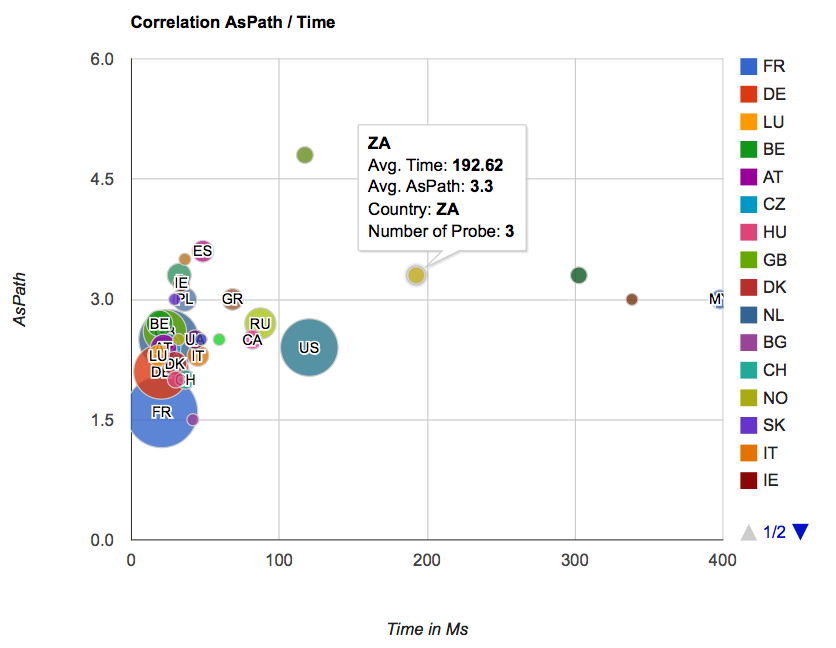
\includegraphics[width=1\linewidth]{illustrations/1-AS-Path-Time-correlation}
	\caption{La corrélation entre la moyenne des AS paths et la moyenne des RTTs \cite{Salim-Gasmi}}
	\label{fig:1-AS-Path-Time-correlationv}
\end{figure}


Ensuite, S. Gasmi a mesuré le RTT entre des sondes Atlas dans le monde et son ancre, il a aussi visualisé le nombre de sauts parcourus entre des sondes Atlas à travers le monde et son ancre. Ces deux visualisations permettent d'avoir une idée sur la latence entre certains pays et le pays de l'ancre en question. Plus de détails sur l'approche sont disponibles dans \cite{Salim-Gasmi}.


\paragraph{La vérification de la cohérence du Traceroute}~

Les chemins parcourus par traceroute pour aller d'une source $s$ vers une destination $d$ changent au cours du temps pour plusieurs raisons. Par exemple, suite   à un changement BGP, à une  répartition des charges, à des pannes des routeurs,  à des pannes des liens physiques, etc.

\textit{Traceroute Consistency Check} peut reprendre les chemins obtenus via traceroute au cours du temps . L'objectif est de suivre les  n\oe{}uds apparaissant dans le chemin allant de  $s$ à $d$ aux instants $t$, $t+1$, $t+2$, etc, et cela afin de voir les n\oe{}uds traversés plus fréquemment au cours du temps. Le chemin est mis à jour via Atlas streaming API. 

L'outil proposé dessine les chemins traceroute comme étant un graphe dirigé, chaque n\oe{}ud est coloré suivant sa cohérence. Le code source du projet est disponible sur GitHub \cite{Traceroute-consistency-check}. La Figure \ref{fig:Traceroute-consistency-check} présente un exemple de la visualisation proposée. Ce résultat concerne la mesure $1663314$ \footnote{Source : \url{https://atlas.ripe.net/measurements/1663314/}, consultée le $05/08/2018$.}. Ce sont des traceroutes à destination de l'adresse $213.171.160.1$, effectués entre le $02/05/2014$ $13:00$ et le $03/05/2014$ $15:00$.

\begin{figure}[H]
	\centering
	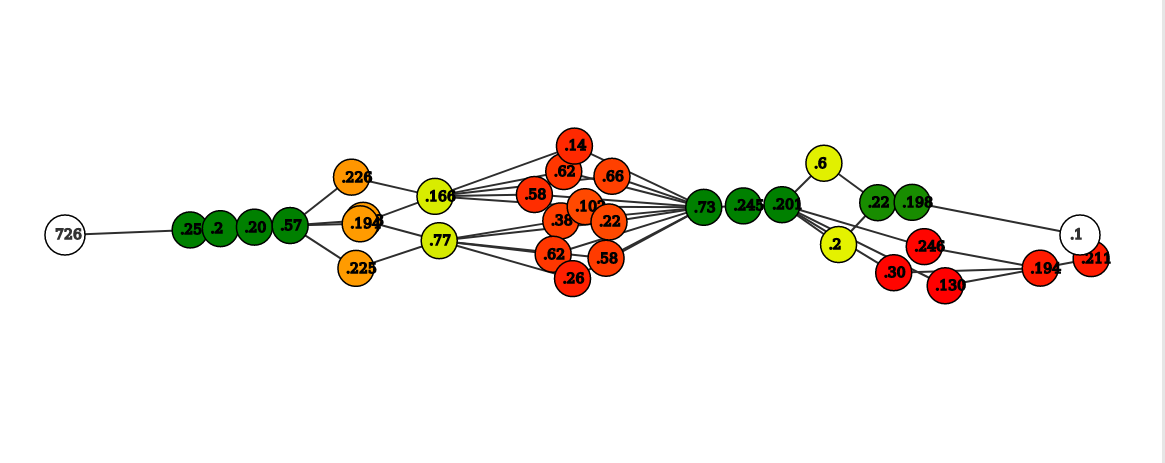
\includegraphics[width=1\linewidth]{illustrations/traceroute-consitance.png}
	\caption{Visualisation des changements des chemins traceroute \cite{Traceroute-consistency-check}}
	\label{fig:Traceroute-consistency-check}
\end{figure}

\paragraph{BGP+traceroute} ~

C'est une combinaison des données BGP (RIPE RIS) et traceroute (RIPE Atlas). L'objectif de ce projet est de partir d'un AS path pour enfin géolocaliser les ASs. 
L'idée est de prendre un AS path des données RIPE RIS, puis, récupérer le préfixe (bloc d'adresses IP) annoncé via cet AS path, ensuite, lancer un traceroute vers une des adresses du bloc. Enfin, géolocaliser les ASs via les données du traceroute. 
Le code source et la présentation de ce projet sont disponibles GitHub \cite{bgp-traceroutes,pres-bgp-traceroute}. 


\paragraph{BGP Atlas Monitor (BAM)} ~

Le projet \textit{BAM} vise la visualisation , en temps réel,  des informations utiles pour les opérateurs des réseaux. Par exemple, BAM montre  la visibilité des préfixes obtenus par RIPE RIS. De plus,  il est possible de voir  le délai du \textit{ping} obtenu via les sondes   Atlas. Le code source est disponible sur  GitHub \cite{bam}. En fournissant un ASN (identifiant d'un AS), \textit{BAM} récupère les préfixes IPv4 et IPv6 et leur visibilité et il montre aussi les sondes dans cet AS. L'outil offre  les  fonctionnalités suivantes :
\begin{itemize}
	\item[--] les préfixes annoncés par un ASN;
	\item[--] la visibilité d'un ASN;
	\item[--] la visibilité d'un préfixe;
	\item[--] la liste des sondes par AS;
	\item[--] les objets  route des préfixes.
\end{itemize}

\paragraph{Prédiction des routeurs provoquant la perte des paquets }~

Dans l'étude \cite{DBLP:journals/corr/FontugneAPB16}, R. Fontugne et al. ont modélisé le comportement  des routeurs, ils ont développé un modèle qui permet d'estimer l'endroit de la  perte des paquets. A partir des traceroutes passant par un routeur \textit{r} à une destination \textit{d}, ils ont construit un modèle de forwarding pour ce routeur. Ce modèle reprend les prochains sauts (routeurs) et la fréquence de passage par ces derniers. Si le routeur \textit{r} change le prochain saut qui a eu "l'habitude" de traverser  pour atteindre \textit{d}, alors cela pour être un indicateur de l'origine  de la perte des paquets.

\subsection{Le suivi des détours dans un trafic local}

Dans leur travail \cite{Emile-Aben-IXP-countries}, E. Aben et al. avaient l'objectif de  voir comment les mesures du RIPE Atlas peuvent fournir un aperçu sur le chemin du trafic local à un pays. Précisément si ce trafic traverse un autre pays en revenant au pays du départ.  Ce qui pourrait  aider à améliorer les performances et l'efficacité des IXPs.  L'objectif est  d'analyser les chemins identifiés dans le trafic d'Internet entre les sondes  Atlas dans un pays donné et essayer d'identifier si le trafic  traverse les IXPs.


France-IX est un point d'échange Internet (IXP) français créé en juin 2010. Afin d'apprendre la topologie de routage, un RIS route collector (RRC21) a été installé au sein du France-IX. Actuellement, la France compte $755$ sondes  Atlas et $9$ ancres. Une ancre sur les $9$ est installée au sein de France-IX.

Une des questions posées c'est de savoir si le trafic local de la France reste localement.  Les sondes  Atlas ne permettent pas de mesurer le trafic entre deux points, alors qu' elles permettent de calculer le chemin entre deux points, adresses IP, ce qui permet d'inférer les sauts par lesquels il passe le trafic. Le travail \cite{France-IX} s'intéresse au trafic depuis et vers une sonde en France en se basant sur l'étude \cite{Emile-Aben-IXP-countries}.


Les résultats obtenus de l'analyse des détours peuvent être intéressants pour les opérateurs des réseaux afin d'améliorer leurs services, ainsi intéressants pour les IXPs tels qu'ils peuvent  proposer des services de peering dans les endroits où il le faut.


\subsection{Visualisation : indicateurs et dashboard}

L'objectif de certains travaux est  d'exploiter les données collectées par les sondes Atlas pour concevoir des tableaux des indicateurs. Par exemple, à partir des données de connexion/déconnexion des sondes Atlas, on peut visualiser les sondes connectées, déconnectées, abandonnées. Un autre projet avait comme objectif la reconstruction d'un graphe reprenant les routeurs (n\oe{}uds) impliqués dans certains traceroutes, ainsi, identifier les n\oe{}uds les plus traversés. D'autres travaux ont repris les détails de la latence, essentiellement, sont les valeurs des RTTs dans les pings et les traceroutes qui permettent de visualiser ce type d'information. 


La liste des travaux basés sur le projet RIPE Atlas est très longue. Nous avons essayé d'énumérer quelques projets, les classer par thèmes, toutefois, ce n'est pas un classement unique, tel qu'on peut retrouver un travail dans plus d'une catégorie, ou bien les classer par un autre classement.

\section{Conclusion}

Dans ce chapitre, nous avons présenté les sondes Atlas et leur fonctionnement, ainsi que quelques travaux ayant impliqué des données collectées par ces sondes.  Ces travaux ont visé différents thèmes, tels que la prise de décision, le suivi des censures, la conception des tableaux de visualisation, etc. Dans le reste de ce document, le choix a été porté sur un sujet lié aux performances des réseaux informatiques. Il s'agit d'un outil de détection des anomalies dans les délais des liens dans les réseaux informatiques, en se basant sur les mesures de traceroute. Une présentation détaillée de l'algorithme de détection est donnée dans le chapitre \ref{chap:algorith-detection}.

%Cet outil donne de meilleure résultat si les données utilisées sont assez grande.  Toutefois, lCependant, ces données sont massives, elles sont  dans l'ordre d'une dizaine de GB rien que pour pour une heure de mesures du type traceroute par exemple, y incluent toutes les destinations.
%C'est pourquoi il faut considérer des outils adaptés. 

%En effet, le chapitre 2 aborde le sujet du Big Data dans ses différentes dimensions. 

%Dans  ce chapitre, nous avons découvert le fonctionnement des sondes Atlas  ainsi que les travaux ayant impliqué les données collectées par ces sondes.  Nous avons appris aussi la nature des données que les sondes Atlas collectent, c'est  crucial pour mener à toute analyse. Vu l'ordre de grandeur de la  quantité de données collectées, les outils traditionnels ne peuvent pas traiter ces données de façon efficace.


%en particulier, à   l'analyse prévue dans le chapitre \ref{chap:implementation}. 

